% Latex header for doxygen 1.8.4
\documentclass[twoside]{book}

% Packages required by doxygen
\usepackage{calc}
\usepackage{doxygen}
\usepackage{graphicx}
\usepackage[utf8]{inputenc}
\usepackage{makeidx}
\usepackage{multicol}
\usepackage{multirow}
\usepackage{textcomp}
\usepackage[table]{xcolor}
\usepackage{epstopdf}
\usepackage{graphics}

% Font selection
\usepackage[T1]{fontenc}
\usepackage{mathptmx}
\usepackage[scaled=.90]{helvet}
\usepackage{courier}
\usepackage{amssymb}
\usepackage{sectsty}
\renewcommand{\familydefault}{\sfdefault}
\allsectionsfont{%
  \fontseries{bc}\selectfont%
  \color{darkgray}%
}
\renewcommand{\DoxyLabelFont}{%
  \fontseries{bc}\selectfont%
  \color{darkgray}%
}

% Page & text layout
\usepackage{geometry}
\geometry{%
  a4paper,%
  top=2.5cm,%
  bottom=2.5cm,%
  left=2.5cm,%
  right=2.5cm%
}
\tolerance=750
\hfuzz=15pt
\hbadness=750
\setlength{\emergencystretch}{15pt}
\setlength{\parindent}{0cm}
\setlength{\parskip}{0.2cm}
\makeatletter
\renewcommand{\paragraph}{%
  \@startsection{paragraph}{4}{0ex}{-1.0ex}{1.0ex}{%
    \normalfont\normalsize\bfseries\SS@parafont%
  }%
}
\renewcommand{\subparagraph}{%
  \@startsection{subparagraph}{5}{0ex}{-1.0ex}{1.0ex}{%
    \normalfont\normalsize\bfseries\SS@subparafont%
  }%
}
\makeatother

% Headers & footers
\usepackage{fancyhdr}
\pagestyle{fancyplain}
\fancyhead[LE]{\fancyplain{}{\bfseries\thepage}}
\fancyhead[CE]{\fancyplain{}{}}
\fancyhead[RE]{\fancyplain{}{\bfseries\leftmark}}
\fancyhead[LO]{\fancyplain{}{\bfseries\rightmark}}
\fancyhead[CO]{\fancyplain{}{}}
\fancyhead[RO]{\fancyplain{}{\bfseries\thepage}}
\fancyfoot[LE]{\fancyplain{}{}}
\fancyfoot[CE]{\fancyplain{}{}}
\fancyfoot[RE]{\fancyplain{}{\bfseries\scriptsize Generated on Sat Jul 20 2013 13:53:46 for My Project by Doxygen }}
\fancyfoot[LO]{\fancyplain{}{\bfseries\scriptsize Generated on Sat Jul 20 2013 13:53:46 for My Project by Doxygen }}
\fancyfoot[CO]{\fancyplain{}{}}
\fancyfoot[RO]{\fancyplain{}{}}
\renewcommand{\footrulewidth}{0.4pt}
\renewcommand{\chaptermark}[1]{%
  \markboth{#1}{}%
}
\renewcommand{\sectionmark}[1]{%
  \markright{\thesection\ #1}%
}

% Indices & bibliography
\usepackage{natbib}
\usepackage[titles]{tocloft}
\setcounter{tocdepth}{3}
\setcounter{secnumdepth}{5}
\makeindex

% Hyperlinks (required, but should be loaded last)
\usepackage{ifpdf}
\ifpdf
  \usepackage[pdftex,pagebackref=true]{hyperref}
\else
  \usepackage[ps2pdf,pagebackref=true]{hyperref}
\fi
\hypersetup{%
  colorlinks=true,%
  linkcolor=blue,%
  citecolor=blue,%
  unicode%
}

% Custom commands
\newcommand{\clearemptydoublepage}{%
  \newpage{\pagestyle{empty}\cleardoublepage}%
}


%===== C O N T E N T S =====

\begin{document}

% Titlepage & ToC
\hypersetup{pageanchor=false}
\pagenumbering{roman}
\begin{titlepage}
\vspace*{7cm}
\begin{center}%
{\Large ezLCD Python Module 1.02}\\
\vspace*{1cm}
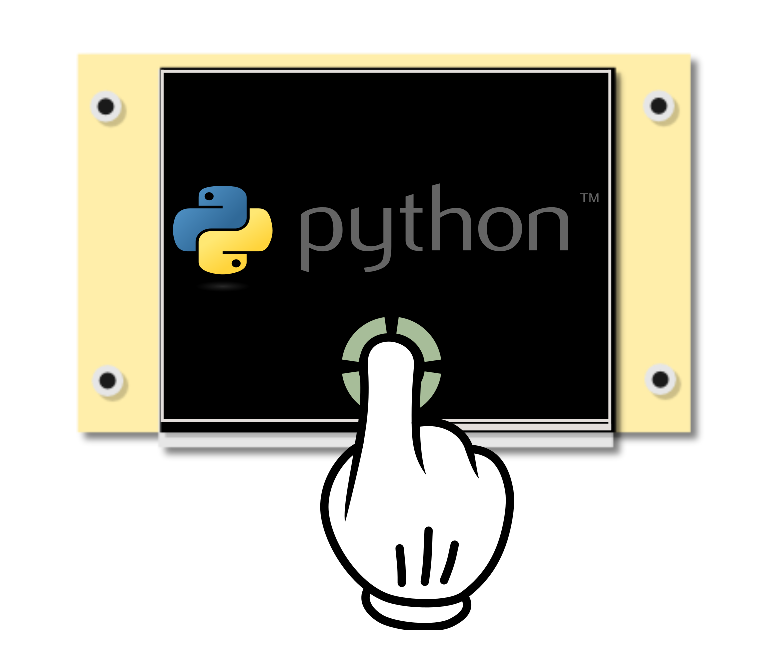
\includegraphics{ezLCDPython.eps}\\
\vspace*{1cm}
{\large Generated by Doxygen 1.8.4}\\
\vspace*{0.5cm}
{\small Sat Jul 20 2013 13:53:46}\\
\end{center}
\end{titlepage}
\clearemptydoublepage
\tableofcontents
\clearemptydoublepage
\pagenumbering{arabic}
\hypersetup{pageanchor=true}

%--- Begin generated contents ---
\chapter{Installing the Module}
\label{install}
\hypertarget{install}{}
install info here\par
 requires py\-Serial \href{http://pyserial.sourceforge.net/}{\tt http\-://pyserial.\-sourceforge.\-net/} 
\chapter{Introduction To The Coordinates System}
\label{coordinatesSystem}
\hypertarget{coordinatesSystem}{}
 
\begin{DoxyImageNoCaption}
  \mbox{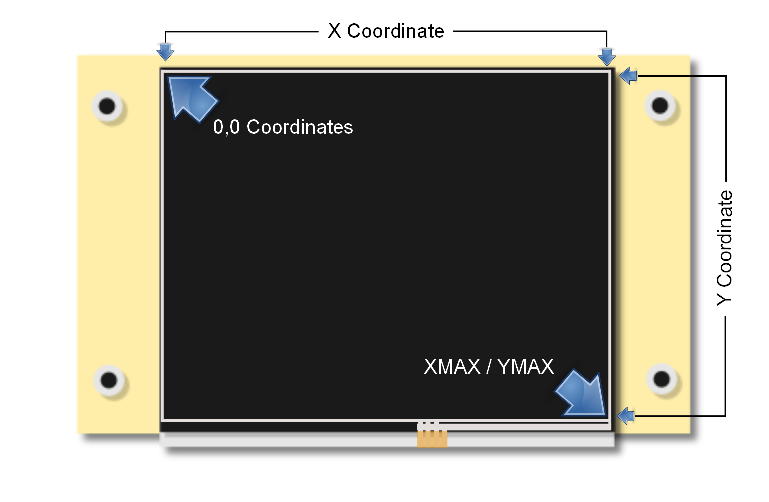
\includegraphics{ezLCD303-coord}}
\end{DoxyImageNoCaption}
 

The ez\-L\-C\-D uses a X Y coordinates system to specify the location for all graphics commands .\par
 {\bfseries One thing to note is that the displays X Y start at 0, so even though you have a display that is 480x272 pixels wide X\-M\-A\-X is 479 and Y\-M\-A\-X is 271.}\par
 X direction is horizontal across the display starting at the left 0 and ending at the max width of the display.\par
 Y direction is vertical starting at the top 0 and ending at the bottom of the display. \par


X\-M\-A\-X and Y\-M\-A\-X Values for the ez\-L\-C\-D 3xx Line\par
 ar\-L\-C\-D 319 239\par
 ez\-L\-C\-D-\/301 399 239\par
 ez\-L\-C\-D-\/302 \par
 ez\-L\-C\-D-\/303 319 239\par
 ez\-L\-C\-D-\/313 319 239\par
 ez\-L\-C\-D-\/304 479 271\par

\chapter{Introduction To The Hardware}
\label{introHardware}
\hypertarget{introHardware}{}
The ez\-L\-C\-D modules contains a G\-P\-U an related circutry to drive a L\-C\-D display, U\-S\-B interface \par
 Internal 4mb M\-S\-D flash drive for storage of fonts, bitmaps and macros.\par
 Display can be controlled through U\-S\-B C\-D\-C Serial or T\-T\-L 3.\-3v Serial .\par
 \par
 Once power is applied to the display it starts up and executes startup.\-ezm, it will look in /\-E\-Z\-U\-S\-E\-R/\-M\-A\-C\-R\-O\-S and if not found will look in /\-E\-Z\-S\-Y\-S/\-U\-S\-E\-R\-S .\par
 What this file does in set all defaults for the Display and communcations port.\par
 Including some default widget fonts and themes. \par
 Its best to have a minimal one in the /\-E\-Z\-U\-S\-E\-R/\-M\-A\-C\-R\-O\-S directory with only the relevent settings in it . \par
 \par
 Sample minimal startup.\-ezm. 
\begin{DoxyCodeInclude}
\textcolor{stringliteral}{'minimal startup.ezm}
\textcolor{stringliteral}{}
\textcolor{stringliteral}{'}Turn off \hyperlink{group___general_ga350c2e1be0d3d074d79d7a7278c44a22}{verbose} echo of commands
\hyperlink{group___general_ga350c2e1be0d3d074d79d7a7278c44a22}{verbose} off

\textcolor{stringliteral}{'Set command port to USB CDC}
\textcolor{stringliteral}{cmd cdc}
\textcolor{stringliteral}{}
\textcolor{stringliteral}{'}\textcolor{keyword}{set} some fonts \textcolor{keywordflow}{for} widgets
\hyperlink{group___widgets_ga0efc2d431900e2b77a30e19bb556fb3a}{fontw} 0 0
\hyperlink{group___widgets_ga0efc2d431900e2b77a30e19bb556fb3a}{fontw} 1 0
\hyperlink{group___widgets_ga0efc2d431900e2b77a30e19bb556fb3a}{fontw} 2 0
\hyperlink{group___widgets_ga0efc2d431900e2b77a30e19bb556fb3a}{fontw} 3 serif24
\hyperlink{group___widgets_ga0efc2d431900e2b77a30e19bb556fb3a}{fontw} 4 serif24
\hyperlink{group___widgets_ga0efc2d431900e2b77a30e19bb556fb3a}{fontw} 5 serif24
\hyperlink{group___widgets_ga0efc2d431900e2b77a30e19bb556fb3a}{fontw} 6 serif24
\hyperlink{group___widgets_ga0efc2d431900e2b77a30e19bb556fb3a}{fontw} 7 serif24

\textcolor{stringliteral}{'Set some themes for widgets}
\textcolor{stringliteral}{theme 0   1   2 0 0 0  3  3   1 0 0}
\textcolor{stringliteral}{theme 1 155 152 3 3 3  24  4   5 0 1}
\textcolor{stringliteral}{theme 2   5  20 3 3 3  4  4   5 0 2}
\textcolor{stringliteral}{theme 3   9   3 0 0 0  8  8   9 0 3}
\textcolor{stringliteral}{theme 4   7   3 0 0 0  6  6   6 6 4}
\textcolor{stringliteral}{theme 5 126 118 3 3 3 35 35  36 0 5}
\textcolor{stringliteral}{theme 6 111 106 3 3 3 12 12 101 0 6}
\textcolor{stringliteral}{theme 7  58  48 3 3 3 14 14  54 0 7}
\textcolor{stringliteral}{}
\textcolor{stringliteral}{color white}
\textcolor{stringliteral}{print "Python CDC Mode 115200 Baud  "}
\textcolor{stringliteral}{'}print device model
print 65
print \textcolor{stringliteral}{"  "}
\textcolor{stringliteral}{'print firmware version}
\textcolor{stringliteral}{print 66}
\end{DoxyCodeInclude}
 The ez\-L\-C\-D by default will load startup.\-ezm but you can have startup1.\-ezm through startup5.\-ezm \par
 So if you press the touch screen at power up in any of the areas show below you can execute the other startup macros.\par
 

 
\begin{DoxyImageNoCaption}
  \mbox{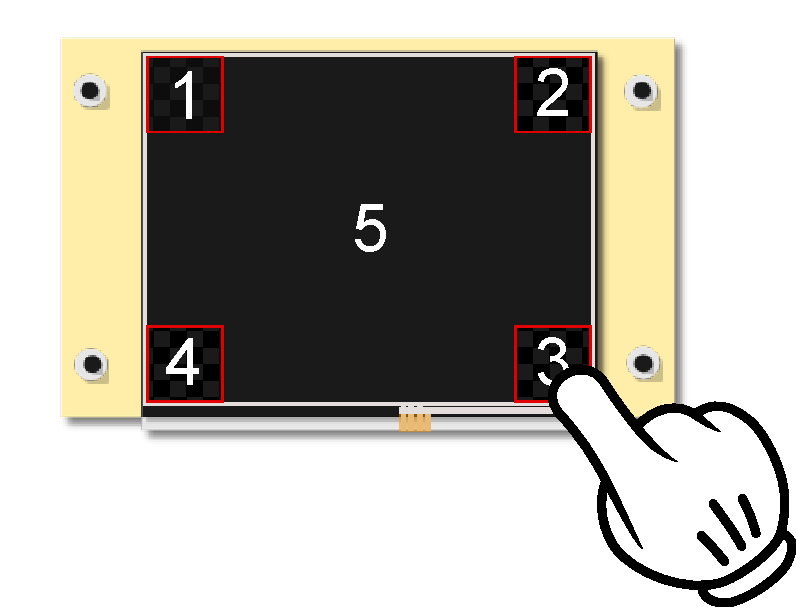
\includegraphics{startupZones}}
\end{DoxyImageNoCaption}
 
\chapter{Introduction To The Software}
\label{introSoftware}
\hypertarget{introSoftware}{}
Commands are sent to the ez\-L\-C\-D though the serial interface, Commands are text based and end with a carrage return {\bfseries cr}.\par
 So if you send {\bfseries cls} ending with a {\bfseries cr} the device will clear the screen and return a {\bfseries cr} when the command is complete,\par
 some widgets take a bit of time (in the millsecond range) to complete so after sending a command allways wait for a {\bfseries cr} to comeback before sending another command.\par
 

\par
 Minimal example will open the ez\-L\-C\-D port clear the screen and print 'Hello From Python' in red \par
  
\begin{DoxyImageNoCaption}
  \mbox{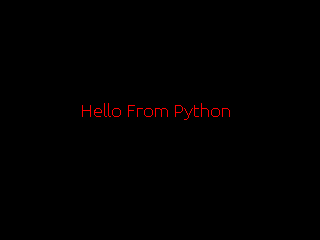
\includegraphics{minimal.png}}
\end{DoxyImageNoCaption}
 
\begin{DoxyCodeInclude}
1 \textcolor{comment}{# Minimal ezLCD Python demo}
2 \textcolor{comment}{#}
3 
4 \textcolor{keyword}{import} platform
5 \textcolor{keyword}{import} sys
6 
7 
8 sys.path.append(\textcolor{stringliteral}{'module'}) 
9 \textcolor{keyword}{from} ezLCD3xx \textcolor{keyword}{import} *
10 
11 LCD = ezLCD(\textcolor{keywordtype}{None}) 
12 comPort =  LCD.findezLCD()
13 
14 \textcolor{comment}{#check what OS we are on}
15 \textcolor{comment}{#Windows}
16 \textcolor{keywordflow}{if} platform.system() == \textcolor{stringliteral}{'Windows'}:
17     LCD = ezLCD(comPort[0][0])
18 \textcolor{comment}{#Mac}
19 \textcolor{keywordflow}{elif} platform.system() == \textcolor{stringliteral}{'Darwin'}:
20     LCD = ezLCD(\textcolor{stringliteral}{'/dev/tty.usbsomething'})
21 \textcolor{comment}{# Bail out if comport error}
22 \textcolor{keywordflow}{if} LCD.openSerial()==\textcolor{keyword}{False}:
23     \textcolor{keywordflow}{print} \textcolor{stringliteral}{'Error Opening Port'}
24     \textcolor{keywordflow}{raise} SystemExit
25 
26 \textcolor{comment}{# Turn verbose off }
27 LCD.verbose(OFF)
28 \textcolor{comment}{# Turn off button press info from ezLCD}
29 LCD.wquiet(ON)
30 \textcolor{comment}{# CLear screen}
31 LCD.cls()
32 \textcolor{comment}{# Set draw color to red}
33 LCD.color(BLUE)
34 \textcolor{comment}{# Print string at coordinates x=80 and y=100}
35 LCD.printString(\textcolor{stringliteral}{"Hello From Python"},80,100)
36 \textcolor{comment}{# Close serial port}
37 LCD.closeSerial()
38 
\end{DoxyCodeInclude}
 
\chapter{Introduction To Themes}
\label{introThemes}
\hypertarget{introThemes}{}
Themes will specify the colors used on widgets (buttons, sliders ect)\par
 The command looks bad but is easy to understand .\par
  
\begin{DoxyImageNoCaption}
  \mbox{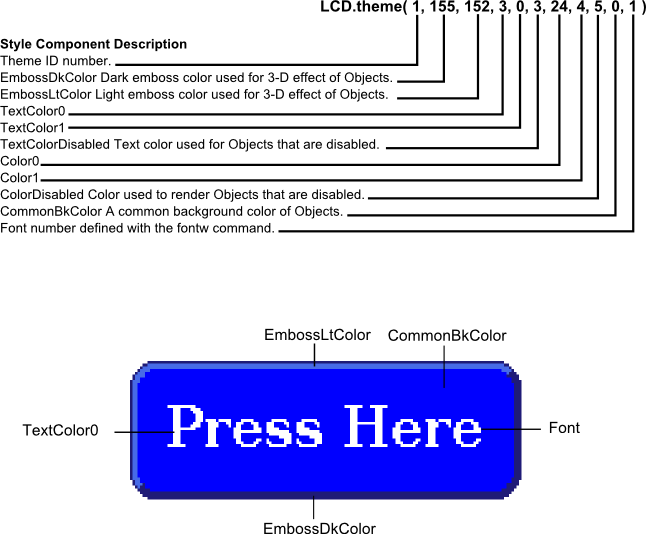
\includegraphics{themes}}
\end{DoxyImageNoCaption}
 
\chapter{Color Table}
\label{colors}
\hypertarget{colors}{}
 
\begin{DoxyImageNoCaption}
  \mbox{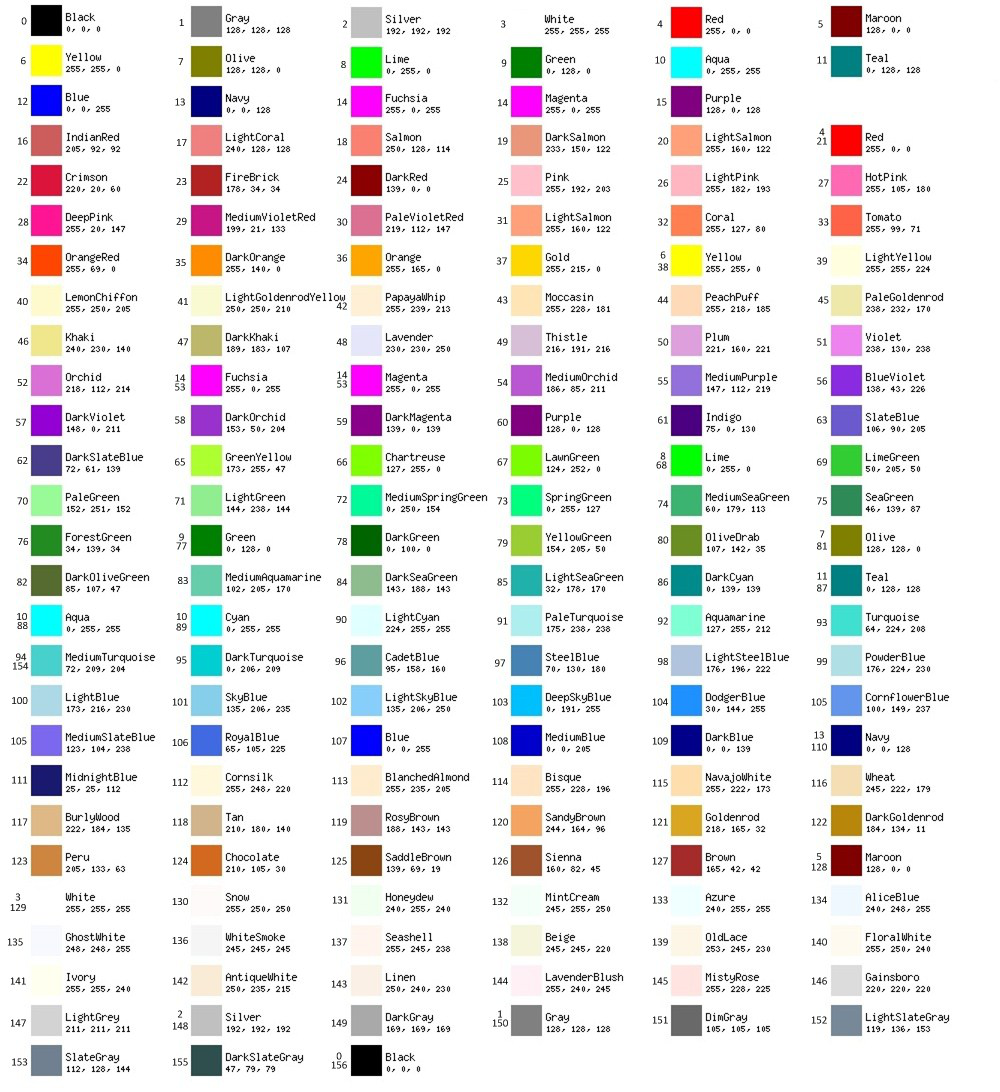
\includegraphics{colors.png}}
\end{DoxyImageNoCaption}
 
\chapter{Introduction To Fonts}
\label{introFonts}
\hypertarget{introFonts}{}
\input{d4/d22/intro_fonts}
\chapter{Introduction To Bitmaps}
\label{introBitmaps}
\hypertarget{introBitmaps}{}
picture supports gif, jpg and bmp
\chapter{Introduction To Widgets}
\label{introWidgets}
\hypertarget{introWidgets}{}
\hypertarget{d0/d90/intro_widgets_overView}{}\section{Over View of Widgets}\label{d0/d90/intro_widgets_overView}
text text\par
 \hypertarget{d0/d90/intro_widgets_buttons}{}\section{Buttons}\label{d0/d90/intro_widgets_buttons}
text text\par
 

 \hypertarget{d0/d90/intro_widgets_touchZone}{}\section{Touch\-Zone}\label{d0/d90/intro_widgets_touchZone}
Touch\-Zones work like buttons but do not display any graphics on their own\par
 You have to supply the image.\par
 So we can take the image below and can make 21 Touch\-Zones one for each Emoticon\par
  \hypertarget{d0/d90/intro_widgets_slider}{}\section{Slider}\label{d0/d90/intro_widgets_slider}
text text\par
 \hypertarget{d0/d90/intro_widgets_progressBar}{}\section{Progress\-Bar}\label{d0/d90/intro_widgets_progressBar}
text text\par
 \hypertarget{d0/d90/intro_widgets_analogMeter}{}\section{Analog\-Meter}\label{d0/d90/intro_widgets_analogMeter}
text text\par
 \hypertarget{d0/d90/intro_widgets_digitalMeter}{}\section{Digital\-Meter}\label{d0/d90/intro_widgets_digitalMeter}
text text\par
 \hypertarget{d0/d90/intro_widgets_staticText}{}\section{Static\-Text}\label{d0/d90/intro_widgets_staticText}
text text\par
 \hypertarget{d0/d90/intro_widgets_groupBox}{}\section{Group\-Box}\label{d0/d90/intro_widgets_groupBox}
text text\par
 \hypertarget{d0/d90/intro_widgets_dial}{}\section{Dial}\label{d0/d90/intro_widgets_dial}
text text\par
 \hypertarget{d0/d90/intro_widgets_choice}{}\section{Choice}\label{d0/d90/intro_widgets_choice}
text text\par
 \hypertarget{d0/d90/intro_widgets_checkBox}{}\section{Check\-Box}\label{d0/d90/intro_widgets_checkBox}
text text\par
 \hypertarget{d0/d90/intro_widgets_radioButtons}{}\section{Radio Buttons}\label{d0/d90/intro_widgets_radioButtons}
text text\par
 
\chapter{Examples}
\label{examples}
\hypertarget{examples}{}
\begin{DoxyVerb}Button example will display a button widget then poll for button presses and update screen <br>
\end{DoxyVerb}
  
\begin{DoxyImageNoCaption}
  \mbox{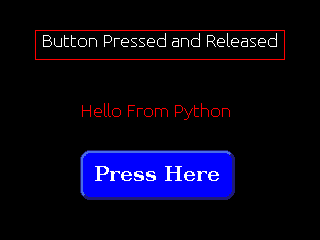
\includegraphics{button.png}}
\end{DoxyImageNoCaption}
 
\begin{DoxyCodeInclude}
1 \textcolor{comment}{# Button ezLCD Python demo}
2 \textcolor{comment}{#}
3 
4 \textcolor{keyword}{import} platform
5 \textcolor{keyword}{import} sys
6 sys.path.append(\textcolor{stringliteral}{'module'}) 
7 \textcolor{keyword}{from} ezLCD3xx \textcolor{keyword}{import} *
8 
9 LCD = ezLCD(\textcolor{keywordtype}{None}) 
10 comPort =  LCD.findezLCD()
11 
12 \textcolor{comment}{#check what OS we are on}
13 \textcolor{comment}{#Windows}
14 \textcolor{keywordflow}{if} platform.system() == \textcolor{stringliteral}{'Windows'}:
15     LCD = ezLCD(comPort[0][0])
16 \textcolor{comment}{#Mac}
17 \textcolor{keywordflow}{elif} platform.system() == \textcolor{stringliteral}{'Dawrwin'}:
18     LCD = ezLCD(\textcolor{stringliteral}{'/dev/tty.usbsomething'})
19 \textcolor{comment}{#Linux}
20 \textcolor{keywordflow}{elif} platform.system() == \textcolor{stringliteral}{'Linux'}:
21     LCD = ezLCD(\textcolor{stringliteral}{'/dev/ttyACM0'})
22 
23 \textcolor{comment}{# Bail out if comport error}
24 \textcolor{keywordflow}{if} LCD.openSerial()==\textcolor{keyword}{False}:
25     \textcolor{keywordflow}{print} \textcolor{stringliteral}{'Error Opening Port'}
26     \textcolor{keywordflow}{raise} SystemExit
27 
28 \textcolor{comment}{# Turn verbose off }
29 LCD.verbose(OFF)
30 \textcolor{comment}{# Turn off button press info from ezLCD}
31 LCD.wquiet(ON)
32 \textcolor{comment}{# CLear screen}
33 LCD.cls()
34 \textcolor{comment}{# Set draw color to red}
35 LCD.color(RED)
36 \textcolor{comment}{# Set widget font 0}
37 LCD.fontw(0,\textcolor{stringliteral}{'1'})
38 \textcolor{comment}{# Set wodget font 1}
39 LCD.fontw(1,\textcolor{stringliteral}{'0'})
40 \textcolor{comment}{# Set theme #1 }
41 LCD.theme(1, 155, 152, 3, 0, 3, 24, 4, 5, 0, 1)
42 \textcolor{comment}{# Print string at coordinates x=80 and y=100}
43 LCD.printString(\textcolor{stringliteral}{"Hello From Python"},80,100)
44 \textcolor{comment}{# Draw button widget with a ID of 1}
45 LCD.button( 1,  80, 150, 155, 50, 1, 0, 10, 6, 3,\textcolor{stringliteral}{'Press Here'})
46 \textcolor{comment}{# Draw a staticText box}
47 LCD.staticText(2, 35, 30, 250, 30, 8, 1, 1,\textcolor{stringliteral}{'Press Button'})
48 \textcolor{comment}{# Clear widget stack}
49 LCD.wstack(CLEAR)
50 \textcolor{keywordflow}{while} \textcolor{keyword}{True}:
51     \textcolor{comment}{# check widget stack this will return widget updates (button press ect.) last in first out order}
52     (ID, Info, Data) = LCD.wstack(FIFO)
53 \textcolor{comment}{#   print ID, Info, Data}
54     \textcolor{comment}{# check if ID = 1 widget 1 and info = pressed }
55     \textcolor{keywordflow}{if} ID == 1 \textcolor{keywordflow}{and} Info == 4:
56         \textcolor{comment}{# clear the stack just to be safe}
57 \textcolor{comment}{#       LCD.wstack(CLEAR)}
58         \textcolor{comment}{# change draw color to yellow}
59         LCD.color(YELLOW)
60         \textcolor{comment}{# change change string 1 for text on static text ID 2}
61         LCD.string(1,\textcolor{stringliteral}{'Button Pressed'})
62         \textcolor{comment}{# redraw static text box ID 2 3=redraw      }
63         LCD.wstate(2, 3)
64     \textcolor{comment}{# check if ID = 1 widget 1 and info = pressed and released}
65     \textcolor{keywordflow}{if} ID == 1 \textcolor{keywordflow}{and} Info == 1:
66         \textcolor{comment}{# clear the stack just to be safe}
67 \textcolor{comment}{#       LCD.wstack(CLEAR)}
68         \textcolor{comment}{# change draw color to yellow}
69         LCD.color(YELLOW)
70         \textcolor{comment}{# change change string 1 for text on static text ID 2}
71         LCD.string(1,\textcolor{stringliteral}{'Button Pressed and Released'})
72         \textcolor{comment}{# redraw static text box ID 2 3=redraw}
73         LCD.wstate(2, 3)
74 
75         
\end{DoxyCodeInclude}
 Load example will display the cpu load as a graph \par
  
\begin{DoxyImageNoCaption}
  \mbox{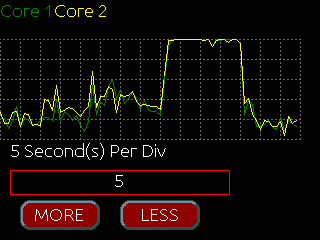
\includegraphics{load.png}}
\end{DoxyImageNoCaption}
 
\begin{DoxyCodeInclude}
1 \textcolor{comment}{#!/usr/bin/env python}
2 \textcolor{comment}{# Python Serial library for ezLCD3xx}
3 \textcolor{comment}{# http://www.ezlcd.com/}
4 \textcolor{comment}{#}
5 \textcolor{comment}{# You need the pySerial Library by Chris Liechti}
6 \textcolor{comment}{# http://pyserial.wiki.sourceforge.net/pySerial}
7 \textcolor{comment}{#}
8 
9 
10 \textcolor{comment}{# END SerLCD Class Definition --------------------------------------}
11 
12 \textcolor{comment}{# Start Test Program -----------------------------------------------}
13 \textcolor{keyword}{import} commands
14 \textcolor{keyword}{import} os
15 \textcolor{keyword}{import} re
16 \textcolor{keyword}{import} time \textcolor{keyword}{as} timer
17 \textcolor{keyword}{import} sys
18 \textcolor{keyword}{import} platform
19 \textcolor{keyword}{import} time
20 \textcolor{keyword}{import} psutil
21     
22 sys.path.append(\textcolor{stringliteral}{'module'}) 
23 \textcolor{keyword}{from} ezLCD3xx \textcolor{keyword}{import} *
24 
25 \textcolor{keyword}{def }drawGrid():
26     LCD.lineType(2)
27     LCD.xy(0,30)
28     LCD.color(BLACK)
29     LCD.box(300,110,1)
30     LCD.xy(0,0)
31     LCD.color(GREEN)
32     LCD.printString(\textcolor{stringliteral}{'Core 1'})
33     LCD.color(YELLOW)
34     LCD.printString(\textcolor{stringliteral}{'  Core 2'})
35     LCD.color(155)
36     LCD.color(LIME)
37     LCD.font(\textcolor{stringliteral}{'1'})
38     LCD.font(\textcolor{stringliteral}{'0'})
39     LCD.color(151)
40     \textcolor{keywordflow}{for} y \textcolor{keywordflow}{in} range(6):
41         LCD.xy(0,(y*20)+39)
42         LCD.line(300,(y*20)+39)
43     \textcolor{keywordflow}{for} x \textcolor{keywordflow}{in} range(16):
44         LCD.xy(x*20,39)
45         LCD.line(x*20,139)
46     LCD.xy(300,39)
47     LCD.line(300,139)
48     LCD.lineType(0)
49     
50 \textcolor{keyword}{def }drawTime(res):
51     LCD.xy(10,140)
52     LCD.color(BLACK)
53     LCD.box(300,30, FILLED)
54     LCD.color(WHITE)
55     Time=str(res)+\textcolor{stringliteral}{' Second(s) Per Div'}
56     LCD.printString(Time)
57 
58     LCD.string(5, str(res))
59     LCD.wstate(7,REDRAW)
60 
61 LCD = ezLCD(\textcolor{keywordtype}{None}) 
62 comPort =  LCD.findezLCD()
63 
64 \textcolor{comment}{#check what OS we are on}
65 \textcolor{comment}{#Windows}
66 \textcolor{keywordflow}{if} platform.system() == \textcolor{stringliteral}{'Windows'}:
67     LCD = ezLCD(comPort[0][0])
68 \textcolor{comment}{#Mac}
69 \textcolor{keywordflow}{elif} platform.system() == \textcolor{stringliteral}{'Dawrwin'}:
70     LCD = ezLCD(\textcolor{stringliteral}{'/dev/tty.usbsomething'})
71 \textcolor{comment}{#Linux}
72 \textcolor{keywordflow}{elif} platform.system() == \textcolor{stringliteral}{'Linux'}:
73     LCD = ezLCD(\textcolor{stringliteral}{'/dev/ttyACM0'})
74 \textcolor{comment}{# Bail out if comport error}
75 \textcolor{keywordflow}{if} LCD.openSerial()==\textcolor{keyword}{False}:
76     \textcolor{keywordflow}{print} \textcolor{stringliteral}{'Error Opening Port'}
77     \textcolor{keywordflow}{raise} SystemExit
78 
79 LCD.ping()
80 LCD.verbose(\textcolor{stringliteral}{'OFF'})
81 LCD.wquiet(ON)
82 LCD.cls()
83 LCD.fontw(0,\textcolor{stringliteral}{'1'})
84 LCD.fontw(1,\textcolor{stringliteral}{'0'})
85 LCD.fontw(2,\textcolor{stringliteral}{'serif24'})
86 LCD.theme(1, 155, 152, 3, 0, 3, 24, 4, 5, 0, 1)
87 LCD.backlight(100, 5, 10)
88 LCD.cls()
89 LCD.font(\textcolor{stringliteral}{'0'})
90 LCD.fonto(0)
91 info = \textcolor{stringliteral}{' '}
92 LCD.string( 1, \textcolor{stringliteral}{'%'})
93 LCD.color(WHITE)
94 LCD.cfgio(8,\textcolor{stringliteral}{'analog'})
95 \textcolor{keywordflow}{print} LCD.xmax()
96 \textcolor{keywordflow}{print} LCD.ymax()
97 \textcolor{keywordflow}{print} LCD.string(65)
98 \textcolor{keywordflow}{print} LCD.string(66)
99 
100 
101 LCD.button( 5, 20, 200, 80, 30 , 1, 0, 10, 1, 2, \textcolor{stringliteral}{'MORE'})
102 LCD.button( 6, 120, 200, 80, 30 , 1, 0, 10, 1, 3, \textcolor{stringliteral}{'LESS'})
103 LCD.staticText(7, 10, 170, 220, 25, 8, 1, 5, \textcolor{stringliteral}{'test'})
104 drawGrid()
105 x=0
106 y1=239
107 y2=239
108 lx=0
109 ly1=239
110 ly2=239
111 res=5
112 drawTime(res)   
113 LCD.wstack(CLEAR)     
114 \textcolor{keywordflow}{while} \textcolor{keyword}{True}:
115 
116     oldinfo = info
117     cores=psutil.cpu\_percent(interval=1, percpu=\textcolor{keyword}{True})
118     y1 = 139 - cores[0]
119     y2 = 139 - cores[1]
120     \textcolor{keywordflow}{if} x!=0:
121         LCD.color(GREEN)
122         LCD.xy(lx,ly1)
123         LCD.line(x, y1)
124         LCD.color(YELLOW)
125         LCD.xy(lx,ly2)
126         LCD.line(x, y2)
127     ly1 = y1
128     ly2 = y2
129     lx = x   
130     x += 20/res
131     
132     \textcolor{keywordflow}{if} x >= 300:
133         x=0
134         y1=239
135         y2=239
136         lx =0
137         ly1 =239
138         ly2 =239
139         drawGrid()
140     (ID, info, data) = LCD.wstack(LIFO)
141     LCD.wstack(CLEAR)
142     \textcolor{keywordflow}{if} ID == 5 \textcolor{keywordflow}{and} info==1:
143         res +=1
144         drawTime(res)  
145     \textcolor{keywordflow}{if} ID == 6 \textcolor{keywordflow}{and} info==1:
146         \textcolor{keywordflow}{if} res > 1:
147             res -=1
148             drawTime(res)
149 LCD.closeSerial()
150 \textcolor{comment}{# End Test Program --------------------------------------}
\end{DoxyCodeInclude}
 
\chapter{Module Index}
\section{Modules}
Here is a list of all modules\-:\begin{DoxyCompactList}
\item \contentsline{section}{Commands}{\pageref{dd/d0a/group___general}}{}
\item \contentsline{section}{Primitve Drawing Commands}{\pageref{d7/df0/group___drawing}}{}
\item \contentsline{section}{Widgets}{\pageref{df/d3e/group___widgets}}{}
\item \contentsline{section}{Bitmaps and Fonts}{\pageref{d2/d7e/group___bitmap_font}}{}
\end{DoxyCompactList}

\chapter{Namespace Index}
\section{Namespace List}
Here is a list of all documented namespaces with brief descriptions\-:\begin{DoxyCompactList}
\item\contentsline{section}{\hyperlink{namespacemodule_1_1ez_l_c_d3xx}{module.\-ez\-L\-C\-D3xx} }{\pageref{d2/d2f/namespacemodule_1_1ez_l_c_d3xx}}{}
\end{DoxyCompactList}

\chapter{Hierarchical Index}
\section{Class Hierarchy}
This inheritance list is sorted roughly, but not completely, alphabetically\-:\begin{DoxyCompactList}
\item object\begin{DoxyCompactList}
\item \contentsline{section}{module.\-ez\-L\-C\-D3xx.\-ez\-L\-C\-D}{\pageref{d0/dec/classmodule_1_1ez_l_c_d3xx_1_1ez_l_c_d}}{}
\end{DoxyCompactList}
\end{DoxyCompactList}

\chapter{Class Index}
\section{Class List}
Here are the classes, structs, unions and interfaces with brief descriptions\-:\begin{DoxyCompactList}
\item\contentsline{section}{\hyperlink{classez_l_c_d3xx_1_1ez_l_c_d}{ez\-L\-C\-D3xx.\-ez\-L\-C\-D} }{\pageref{d0/dc0/classez_l_c_d3xx_1_1ez_l_c_d}}{}
\end{DoxyCompactList}

\chapter{Module Documentation}
\hypertarget{group___general}{\section{Commands}
\label{dd/d0a/group___general}\index{Commands@{Commands}}
}
\subsection*{Functions}
\begin{DoxyCompactItemize}
\item 
def \hyperlink{group___general_gaa497e8573c045944d589b17fd7dd36ac}{ez\-L\-C\-D3xx.\-verbose}
\begin{DoxyCompactList}\small\item\em The Verbose command will turn on or off more verbose errors. \end{DoxyCompactList}\item 
def \hyperlink{group___general_gabe06f9371514b4556accd06145b9c104}{ez\-L\-C\-D3xx.\-xmax}
\begin{DoxyCompactList}\small\item\em The xmax command will return the max x of current display. \end{DoxyCompactList}\item 
def \hyperlink{group___general_gabcb8010d7c29b1c514e70cefe3bb856c}{ez\-L\-C\-D3xx.\-ymax}
\begin{DoxyCompactList}\small\item\em The ymax command will return the max y of current display. \end{DoxyCompactList}\item 
def \hyperlink{group___general_ga92454899475445ff2d48eb7072f3c94e}{ez\-L\-C\-D3xx.\-ping}
\begin{DoxyCompactList}\small\item\em the ping command \end{DoxyCompactList}\item 
def \hyperlink{group___general_gacecf5c1b5956caef4a4030f51bc4a809}{ez\-L\-C\-D3xx.\-backlight}
\begin{DoxyCompactList}\small\item\em The backlight command will set backlight brightness and timeout. \end{DoxyCompactList}\item 
def \hyperlink{group___general_ga78b38855b8bcb0609d340a80210a0d0f}{ez\-L\-C\-D3xx.\-wquiet}
\begin{DoxyCompactList}\small\item\em The wquiet command disables the touch event data being sent to the console port. \end{DoxyCompactList}\item 
def \hyperlink{group___general_ga38687b7d07bf93afe6891d3dca6205f4}{ez\-L\-C\-D3xx.\-cfgio}
\begin{DoxyCompactList}\small\item\em The cfgio command will configure io pins. \end{DoxyCompactList}\item 
def \hyperlink{group___general_gaf87ad0b88f8a279c20666363bc7460b6}{ez\-L\-C\-D3xx.\-io}
\begin{DoxyCompactList}\small\item\em The io command use to set and clear io pins. \end{DoxyCompactList}\item 
def \hyperlink{group___general_ga15f87f284189816d98ab5bf0b5a94a99}{ez\-L\-C\-D3xx.\-play}
\begin{DoxyCompactList}\small\item\em The play command will play a macro stored on the drive of the \hyperlink{classez_l_c_d3xx_1_1ez_l_c_d}{ez\-L\-C\-D}. \end{DoxyCompactList}\item 
def \hyperlink{group___general_ga7faa11f7fbe4da6ba981a5b8c4cb37aa}{ez\-L\-C\-D3xx.\-run}
\begin{DoxyCompactList}\small\item\em The run command will run a macro stored on the drive of the \hyperlink{classez_l_c_d3xx_1_1ez_l_c_d}{ez\-L\-C\-D}. \end{DoxyCompactList}\item 
def \hyperlink{group___general_gabc1cd3bb62dfa8a8f37f5da5cbb3e85c}{ez\-L\-C\-D3xx.\-reset}
\begin{DoxyCompactList}\small\item\em The reset command will reset the \hyperlink{classez_l_c_d3xx_1_1ez_l_c_d}{ez\-L\-C\-D} and run startup.\-ezm same as power up. \end{DoxyCompactList}\item 
def \hyperlink{group___general_ga8a1ef000b3c71704260c9e5f949e80de}{ez\-L\-C\-D3xx.\-snapshot}
\begin{DoxyCompactList}\small\item\em The snapshot command will write a copy of the current display to the flash drive as a bmp. \end{DoxyCompactList}\end{DoxyCompactItemize}


\subsection{Detailed Description}


\subsection{Function Documentation}
\hypertarget{group___general_gacecf5c1b5956caef4a4030f51bc4a809}{\index{Commands@{Commands}!backlight@{backlight}}
\index{backlight@{backlight}!Commands@{Commands}}
\subsubsection[{backlight}]{\setlength{\rightskip}{0pt plus 5cm}def ez\-L\-C\-D3xx.\-backlight (
\begin{DoxyParamCaption}
\item[{}]{self, }
\item[{}]{brightness, }
\item[{}]{timeout = {\ttfamily None}, }
\item[{}]{level = {\ttfamily None}}
\end{DoxyParamCaption}
)}}\label{dd/d0a/group___general_gacecf5c1b5956caef4a4030f51bc4a809}


The backlight command will set backlight brightness and timeout. 


\begin{DoxyParams}{Parameters}
{\em brightness} & 1 \\
\hline
{\em timeout} & 2 \\
\hline
{\em level} & 3 \\
\hline
\end{DoxyParams}
\hypertarget{group___general_ga38687b7d07bf93afe6891d3dca6205f4}{\index{Commands@{Commands}!cfgio@{cfgio}}
\index{cfgio@{cfgio}!Commands@{Commands}}
\subsubsection[{cfgio}]{\setlength{\rightskip}{0pt plus 5cm}def ez\-L\-C\-D3xx.\-cfgio (
\begin{DoxyParamCaption}
\item[{}]{self, }
\item[{}]{pin, }
\item[{}]{function}
\end{DoxyParamCaption}
)}}\label{dd/d0a/group___general_ga38687b7d07bf93afe6891d3dca6205f4}


The cfgio command will configure io pins. 


\begin{DoxyParams}{Parameters}
{\em pin} & \\
\hline
{\em function} & \\
\hline
\end{DoxyParams}
\hypertarget{group___general_gaf87ad0b88f8a279c20666363bc7460b6}{\index{Commands@{Commands}!io@{io}}
\index{io@{io}!Commands@{Commands}}
\subsubsection[{io}]{\setlength{\rightskip}{0pt plus 5cm}def ez\-L\-C\-D3xx.\-io (
\begin{DoxyParamCaption}
\item[{}]{self, }
\item[{}]{pin, }
\item[{}]{level}
\end{DoxyParamCaption}
)}}\label{dd/d0a/group___general_gaf87ad0b88f8a279c20666363bc7460b6}


The io command use to set and clear io pins. 


\begin{DoxyParams}{Parameters}
{\em pin} & \\
\hline
{\em level} & \\
\hline
\end{DoxyParams}
\hypertarget{group___general_ga92454899475445ff2d48eb7072f3c94e}{\index{Commands@{Commands}!ping@{ping}}
\index{ping@{ping}!Commands@{Commands}}
\subsubsection[{ping}]{\setlength{\rightskip}{0pt plus 5cm}def ez\-L\-C\-D3xx.\-ping (
\begin{DoxyParamCaption}
\item[{}]{self}
\end{DoxyParamCaption}
)}}\label{dd/d0a/group___general_ga92454899475445ff2d48eb7072f3c94e}


the ping command 

\begin{DoxyReturn}{Returns}
0 
\end{DoxyReturn}
\hypertarget{group___general_ga15f87f284189816d98ab5bf0b5a94a99}{\index{Commands@{Commands}!play@{play}}
\index{play@{play}!Commands@{Commands}}
\subsubsection[{play}]{\setlength{\rightskip}{0pt plus 5cm}def ez\-L\-C\-D3xx.\-play (
\begin{DoxyParamCaption}
\item[{}]{self, }
\item[{}]{filename}
\end{DoxyParamCaption}
)}}\label{dd/d0a/group___general_ga15f87f284189816d98ab5bf0b5a94a99}


The play command will play a macro stored on the drive of the \hyperlink{classez_l_c_d3xx_1_1ez_l_c_d}{ez\-L\-C\-D}. 


\begin{DoxyParams}{Parameters}
{\em macro} & filename \\
\hline
\end{DoxyParams}
\hypertarget{group___general_gabc1cd3bb62dfa8a8f37f5da5cbb3e85c}{\index{Commands@{Commands}!reset@{reset}}
\index{reset@{reset}!Commands@{Commands}}
\subsubsection[{reset}]{\setlength{\rightskip}{0pt plus 5cm}def ez\-L\-C\-D3xx.\-reset (
\begin{DoxyParamCaption}
\item[{}]{self}
\end{DoxyParamCaption}
)}}\label{dd/d0a/group___general_gabc1cd3bb62dfa8a8f37f5da5cbb3e85c}


The reset command will reset the \hyperlink{classez_l_c_d3xx_1_1ez_l_c_d}{ez\-L\-C\-D} and run startup.\-ezm same as power up. 

\hypertarget{group___general_ga7faa11f7fbe4da6ba981a5b8c4cb37aa}{\index{Commands@{Commands}!run@{run}}
\index{run@{run}!Commands@{Commands}}
\subsubsection[{run}]{\setlength{\rightskip}{0pt plus 5cm}def ez\-L\-C\-D3xx.\-run (
\begin{DoxyParamCaption}
\item[{}]{self, }
\item[{}]{filename}
\end{DoxyParamCaption}
)}}\label{dd/d0a/group___general_ga7faa11f7fbe4da6ba981a5b8c4cb37aa}


The run command will run a macro stored on the drive of the \hyperlink{classez_l_c_d3xx_1_1ez_l_c_d}{ez\-L\-C\-D}. 


\begin{DoxyParams}{Parameters}
{\em macro} & filename \\
\hline
\end{DoxyParams}
\hypertarget{group___general_ga8a1ef000b3c71704260c9e5f949e80de}{\index{Commands@{Commands}!snapshot@{snapshot}}
\index{snapshot@{snapshot}!Commands@{Commands}}
\subsubsection[{snapshot}]{\setlength{\rightskip}{0pt plus 5cm}def ez\-L\-C\-D3xx.\-snapshot (
\begin{DoxyParamCaption}
\item[{}]{self, }
\item[{}]{x, }
\item[{}]{y, }
\item[{}]{w, }
\item[{}]{h, }
\item[{}]{filename}
\end{DoxyParamCaption}
)}}\label{dd/d0a/group___general_ga8a1ef000b3c71704260c9e5f949e80de}


The snapshot command will write a copy of the current display to the flash drive as a bmp. 


\begin{DoxyParams}{Parameters}
{\em x} & \\
\hline
{\em y} & \\
\hline
{\em w} & \\
\hline
{\em h} & \\
\hline
{\em filename.\-bmp} & \\
\hline
\end{DoxyParams}
\hypertarget{group___general_gaa497e8573c045944d589b17fd7dd36ac}{\index{Commands@{Commands}!verbose@{verbose}}
\index{verbose@{verbose}!Commands@{Commands}}
\subsubsection[{verbose}]{\setlength{\rightskip}{0pt plus 5cm}def ez\-L\-C\-D3xx.\-verbose (
\begin{DoxyParamCaption}
\item[{}]{self, }
\item[{}]{state}
\end{DoxyParamCaption}
)}}\label{dd/d0a/group___general_gaa497e8573c045944d589b17fd7dd36ac}


The Verbose command will turn on or off more verbose errors. 


\begin{DoxyParams}{Parameters}
{\em state} & 0=off 1=on \\
\hline
\end{DoxyParams}
\hypertarget{group___general_ga78b38855b8bcb0609d340a80210a0d0f}{\index{Commands@{Commands}!wquiet@{wquiet}}
\index{wquiet@{wquiet}!Commands@{Commands}}
\subsubsection[{wquiet}]{\setlength{\rightskip}{0pt plus 5cm}def ez\-L\-C\-D3xx.\-wquiet (
\begin{DoxyParamCaption}
\item[{}]{self, }
\item[{}]{state}
\end{DoxyParamCaption}
)}}\label{dd/d0a/group___general_ga78b38855b8bcb0609d340a80210a0d0f}


The wquiet command disables the touch event data being sent to the console port. 


\begin{DoxyParams}{Parameters}
{\em state} & 0=off 1=on \\
\hline
\end{DoxyParams}
\hypertarget{group___general_gabe06f9371514b4556accd06145b9c104}{\index{Commands@{Commands}!xmax@{xmax}}
\index{xmax@{xmax}!Commands@{Commands}}
\subsubsection[{xmax}]{\setlength{\rightskip}{0pt plus 5cm}def ez\-L\-C\-D3xx.\-xmax (
\begin{DoxyParamCaption}
\item[{}]{self}
\end{DoxyParamCaption}
)}}\label{dd/d0a/group___general_gabe06f9371514b4556accd06145b9c104}


The xmax command will return the max x of current display. 

\begin{DoxyReturn}{Returns}
x-\/horizontal resolution in pixels starting from 0 
\end{DoxyReturn}
\hypertarget{group___general_gabcb8010d7c29b1c514e70cefe3bb856c}{\index{Commands@{Commands}!ymax@{ymax}}
\index{ymax@{ymax}!Commands@{Commands}}
\subsubsection[{ymax}]{\setlength{\rightskip}{0pt plus 5cm}def ez\-L\-C\-D3xx.\-ymax (
\begin{DoxyParamCaption}
\item[{}]{self}
\end{DoxyParamCaption}
)}}\label{dd/d0a/group___general_gabcb8010d7c29b1c514e70cefe3bb856c}


The ymax command will return the max y of current display. 

\begin{DoxyReturn}{Returns}
y-\/vertical resolution in pixels starting from 0 
\end{DoxyReturn}

\hypertarget{group___drawing}{\section{Primitve Drawing Commands}
\label{d7/df0/group___drawing}\index{Primitve Drawing Commands@{Primitve Drawing Commands}}
}
\subsection*{Functions}
\begin{DoxyCompactItemize}
\item 
def \hyperlink{group___drawing_gacdfb97b09494d0e3cec787014c4863f9}{ez\-L\-C\-D3xx.\-cls}
\begin{DoxyCompactList}\small\item\em The cls command will clear the screen to black it no color is given. \end{DoxyCompactList}\item 
def \hyperlink{group___drawing_ga306a0e99b15bc1122683a1c6e18e7ef0}{ez\-L\-C\-D3xx.\-color}
\begin{DoxyCompactList}\small\item\em The color command see \hyperlink{namespaceez_l_c_d3xx}{ez\-L\-C\-D3xx} manual for colors. \end{DoxyCompactList}\item 
def \hyperlink{group___drawing_ga94dd8d046a01670fc2212b548e29e8d0}{ez\-L\-C\-D3xx.\-color\-Id}
\begin{DoxyCompactList}\small\item\em The color\-Id command. \end{DoxyCompactList}\item 
def \hyperlink{group___drawing_gaf249f02b6ad4e734ffa9d8371f6cab8a}{ez\-L\-C\-D3xx.\-xy}
\begin{DoxyCompactList}\small\item\em The xy command will set or return the x y coordinates. \end{DoxyCompactList}\item 
def \hyperlink{group___drawing_gad3c0ce418a0feea4a0fa40f803c90196}{ez\-L\-C\-D3xx.\-plot}
\begin{DoxyCompactList}\small\item\em The plot command will set a pixel to current color and if used x y. \end{DoxyCompactList}\item 
def \hyperlink{group___drawing_ga9dc821ce2652535899c584d4ff1c1bf7}{ez\-L\-C\-D3xx.\-line\-Type}
\begin{DoxyCompactList}\small\item\em The line\-Type Command will set the line type for the line command. \end{DoxyCompactList}\item 
def \hyperlink{group___drawing_ga87b2625e7e4ffa927b4471003f8c6e70}{ez\-L\-C\-D3xx.\-line\-Width}
\begin{DoxyCompactList}\small\item\em The line\-Width Command will set the line width for the line command. \end{DoxyCompactList}\item 
def \hyperlink{group___drawing_gae70c22a0a810a70a0dd6d32c9fd7c066}{ez\-L\-C\-D3xx.\-line}
\begin{DoxyCompactList}\small\item\em The line command will draw a line from current xy to line(x,y) \end{DoxyCompactList}\item 
def \hyperlink{group___drawing_ga63bb01e1f5ef0fe2ae2acec0ed90e5bd}{ez\-L\-C\-D3xx.\-box}
\begin{DoxyCompactList}\small\item\em The box command will draw a box starting from the current xy in width and height with option for filled. \end{DoxyCompactList}\item 
def \hyperlink{group___drawing_gabfcfb31f2d88c7397332abcc6b324c7c}{ez\-L\-C\-D3xx.\-circle}
\item 
def \hyperlink{group___drawing_ga12fb93d2d6f7ce3f08ad988c09624d57}{ez\-L\-C\-D3xx.\-pie}
\item 
def \hyperlink{group___drawing_ga13a0a8fb9c906a687f2a42864d973cc1}{ez\-L\-C\-D3xx.\-arc}
\item 
def \hyperlink{group___drawing_ga2f55674143f1e4b06e42f09aaf0da71c}{ez\-L\-C\-D3xx.\-clip\-Area}
\item 
def \hyperlink{group___drawing_gabd1433160288289495e6c006e77951e6}{ez\-L\-C\-D3xx.\-clip\-Enable}
\end{DoxyCompactItemize}


\subsection{Detailed Description}


\subsection{Function Documentation}
\hypertarget{group___drawing_ga13a0a8fb9c906a687f2a42864d973cc1}{\index{Primitve Drawing Commands@{Primitve Drawing Commands}!arc@{arc}}
\index{arc@{arc}!Primitve Drawing Commands@{Primitve Drawing Commands}}
\subsubsection[{arc}]{\setlength{\rightskip}{0pt plus 5cm}def ez\-L\-C\-D3xx.\-arc (
\begin{DoxyParamCaption}
\item[{}]{self, }
\item[{}]{radius, }
\item[{}]{start, }
\item[{}]{end, }
\item[{}]{fill = {\ttfamily 0}}
\end{DoxyParamCaption}
)}}\label{d7/df0/group___drawing_ga13a0a8fb9c906a687f2a42864d973cc1}
\begin{DoxyVerb}The ARC command draws an arc at current XY position. Replace {R} with the desired radius of the arc, in pixels.
fill =1 will draw a filled circle
\end{DoxyVerb}
 \hypertarget{group___drawing_ga63bb01e1f5ef0fe2ae2acec0ed90e5bd}{\index{Primitve Drawing Commands@{Primitve Drawing Commands}!box@{box}}
\index{box@{box}!Primitve Drawing Commands@{Primitve Drawing Commands}}
\subsubsection[{box}]{\setlength{\rightskip}{0pt plus 5cm}def ez\-L\-C\-D3xx.\-box (
\begin{DoxyParamCaption}
\item[{}]{self, }
\item[{}]{width, }
\item[{}]{height, }
\item[{}]{fill = {\ttfamily 0}}
\end{DoxyParamCaption}
)}}\label{d7/df0/group___drawing_ga63bb01e1f5ef0fe2ae2acec0ed90e5bd}


The box command will draw a box starting from the current xy in width and height with option for filled. 


\begin{DoxyParams}{Parameters}
{\em width} & width of box in pixels \\
\hline
{\em height} & height of box in pixels \\
\hline
{\em fill} & 1=filled box 0=outline only $\ast$optional defaults to outline \\
\hline
\end{DoxyParams}
\hypertarget{group___drawing_gabfcfb31f2d88c7397332abcc6b324c7c}{\index{Primitve Drawing Commands@{Primitve Drawing Commands}!circle@{circle}}
\index{circle@{circle}!Primitve Drawing Commands@{Primitve Drawing Commands}}
\subsubsection[{circle}]{\setlength{\rightskip}{0pt plus 5cm}def ez\-L\-C\-D3xx.\-circle (
\begin{DoxyParamCaption}
\item[{}]{self, }
\item[{}]{width, }
\item[{}]{radius, }
\item[{}]{fill = {\ttfamily 0}}
\end{DoxyParamCaption}
)}}\label{d7/df0/group___drawing_gabfcfb31f2d88c7397332abcc6b324c7c}
\begin{DoxyVerb}draw a circle with radius in pixels
fill =1 will draw a filled circle
\end{DoxyVerb}
 \hypertarget{group___drawing_ga2f55674143f1e4b06e42f09aaf0da71c}{\index{Primitve Drawing Commands@{Primitve Drawing Commands}!clip\-Area@{clip\-Area}}
\index{clip\-Area@{clip\-Area}!Primitve Drawing Commands@{Primitve Drawing Commands}}
\subsubsection[{clip\-Area}]{\setlength{\rightskip}{0pt plus 5cm}def ez\-L\-C\-D3xx.\-clip\-Area (
\begin{DoxyParamCaption}
\item[{}]{self, }
\item[{}]{left, }
\item[{}]{top, }
\item[{}]{right, }
\item[{}]{bottom}
\end{DoxyParamCaption}
)}}\label{d7/df0/group___drawing_ga2f55674143f1e4b06e42f09aaf0da71c}

\begin{DoxyParams}{Parameters}
{\em left} & \\
\hline
{\em top} & \\
\hline
{\em right} & \\
\hline
{\em bottom} & \\
\hline
\end{DoxyParams}
\hypertarget{group___drawing_gabd1433160288289495e6c006e77951e6}{\index{Primitve Drawing Commands@{Primitve Drawing Commands}!clip\-Enable@{clip\-Enable}}
\index{clip\-Enable@{clip\-Enable}!Primitve Drawing Commands@{Primitve Drawing Commands}}
\subsubsection[{clip\-Enable}]{\setlength{\rightskip}{0pt plus 5cm}def ez\-L\-C\-D3xx.\-clip\-Enable (
\begin{DoxyParamCaption}
\item[{}]{self, }
\item[{}]{enable}
\end{DoxyParamCaption}
)}}\label{d7/df0/group___drawing_gabd1433160288289495e6c006e77951e6}

\begin{DoxyParams}{Parameters}
{\em enable} & 0=off 1=on \\
\hline
\end{DoxyParams}
\hypertarget{group___drawing_gacdfb97b09494d0e3cec787014c4863f9}{\index{Primitve Drawing Commands@{Primitve Drawing Commands}!cls@{cls}}
\index{cls@{cls}!Primitve Drawing Commands@{Primitve Drawing Commands}}
\subsubsection[{cls}]{\setlength{\rightskip}{0pt plus 5cm}def ez\-L\-C\-D3xx.\-cls (
\begin{DoxyParamCaption}
\item[{}]{self, }
\item[{}]{Color = {\ttfamily None}}
\end{DoxyParamCaption}
)}}\label{d7/df0/group___drawing_gacdfb97b09494d0e3cec787014c4863f9}


The cls command will clear the screen to black it no color is given. 


\begin{DoxyParams}{Parameters}
{\em Color} & color to clear screen to \\
\hline
\end{DoxyParams}
\hypertarget{group___drawing_ga306a0e99b15bc1122683a1c6e18e7ef0}{\index{Primitve Drawing Commands@{Primitve Drawing Commands}!color@{color}}
\index{color@{color}!Primitve Drawing Commands@{Primitve Drawing Commands}}
\subsubsection[{color}]{\setlength{\rightskip}{0pt plus 5cm}def ez\-L\-C\-D3xx.\-color (
\begin{DoxyParamCaption}
\item[{}]{self, }
\item[{}]{color = {\ttfamily None}}
\end{DoxyParamCaption}
)}}\label{d7/df0/group___drawing_ga306a0e99b15bc1122683a1c6e18e7ef0}


The color command see \hyperlink{namespaceez_l_c_d3xx}{ez\-L\-C\-D3xx} manual for colors. 


\begin{DoxyParams}{Parameters}
{\em color} & number \\
\hline
\end{DoxyParams}
\begin{DoxyReturn}{Returns}
color as a tuple 
\end{DoxyReturn}
\hypertarget{group___drawing_ga94dd8d046a01670fc2212b548e29e8d0}{\index{Primitve Drawing Commands@{Primitve Drawing Commands}!color\-Id@{color\-Id}}
\index{color\-Id@{color\-Id}!Primitve Drawing Commands@{Primitve Drawing Commands}}
\subsubsection[{color\-Id}]{\setlength{\rightskip}{0pt plus 5cm}def ez\-L\-C\-D3xx.\-color\-Id (
\begin{DoxyParamCaption}
\item[{}]{self, }
\item[{}]{I\-D, }
\item[{}]{R = {\ttfamily None}, }
\item[{}]{G = {\ttfamily None}, }
\item[{}]{B = {\ttfamily None}}
\end{DoxyParamCaption}
)}}\label{d7/df0/group___drawing_ga94dd8d046a01670fc2212b548e29e8d0}


The color\-Id command. 


\begin{DoxyParams}{Parameters}
{\em R} & \\
\hline
{\em G} & \\
\hline
{\em B} & \\
\hline
\end{DoxyParams}
\begin{DoxyReturn}{Returns}
color as a tuple 
\end{DoxyReturn}
\hypertarget{group___drawing_gae70c22a0a810a70a0dd6d32c9fd7c066}{\index{Primitve Drawing Commands@{Primitve Drawing Commands}!line@{line}}
\index{line@{line}!Primitve Drawing Commands@{Primitve Drawing Commands}}
\subsubsection[{line}]{\setlength{\rightskip}{0pt plus 5cm}def ez\-L\-C\-D3xx.\-line (
\begin{DoxyParamCaption}
\item[{}]{self, }
\item[{}]{x, }
\item[{}]{y}
\end{DoxyParamCaption}
)}}\label{d7/df0/group___drawing_gae70c22a0a810a70a0dd6d32c9fd7c066}


The line command will draw a line from current xy to line(x,y) 


\begin{DoxyParams}{Parameters}
{\em x} & \\
\hline
{\em y} & \\
\hline
\end{DoxyParams}
\hypertarget{group___drawing_ga9dc821ce2652535899c584d4ff1c1bf7}{\index{Primitve Drawing Commands@{Primitve Drawing Commands}!line\-Type@{line\-Type}}
\index{line\-Type@{line\-Type}!Primitve Drawing Commands@{Primitve Drawing Commands}}
\subsubsection[{line\-Type}]{\setlength{\rightskip}{0pt plus 5cm}def ez\-L\-C\-D3xx.\-line\-Type (
\begin{DoxyParamCaption}
\item[{}]{self, }
\item[{}]{option}
\end{DoxyParamCaption}
)}}\label{d7/df0/group___drawing_ga9dc821ce2652535899c584d4ff1c1bf7}


The line\-Type Command will set the line type for the line command. 


\begin{DoxyParams}{Parameters}
{\em option} & 0 = solid, 1= dotted (1 pixel spacing between dots), 2 = dashed (2 pixel spacing between dashes) \\
\hline
\end{DoxyParams}
\hypertarget{group___drawing_ga87b2625e7e4ffa927b4471003f8c6e70}{\index{Primitve Drawing Commands@{Primitve Drawing Commands}!line\-Width@{line\-Width}}
\index{line\-Width@{line\-Width}!Primitve Drawing Commands@{Primitve Drawing Commands}}
\subsubsection[{line\-Width}]{\setlength{\rightskip}{0pt plus 5cm}def ez\-L\-C\-D3xx.\-line\-Width (
\begin{DoxyParamCaption}
\item[{}]{self, }
\item[{}]{width}
\end{DoxyParamCaption}
)}}\label{d7/df0/group___drawing_ga87b2625e7e4ffa927b4471003f8c6e70}


The line\-Width Command will set the line width for the line command. 


\begin{DoxyParams}{Parameters}
{\em width} & thin line (width = 1) or a thick line (width =3). Only \mbox{[}width\mbox{]} = 1 or 3 are available. \\
\hline
\end{DoxyParams}
\hypertarget{group___drawing_ga12fb93d2d6f7ce3f08ad988c09624d57}{\index{Primitve Drawing Commands@{Primitve Drawing Commands}!pie@{pie}}
\index{pie@{pie}!Primitve Drawing Commands@{Primitve Drawing Commands}}
\subsubsection[{pie}]{\setlength{\rightskip}{0pt plus 5cm}def ez\-L\-C\-D3xx.\-pie (
\begin{DoxyParamCaption}
\item[{}]{self, }
\item[{}]{radius, }
\item[{}]{start, }
\item[{}]{end}
\end{DoxyParamCaption}
)}}\label{d7/df0/group___drawing_ga12fb93d2d6f7ce3f08ad988c09624d57}
\begin{DoxyVerb}The PIE command draws a section of a circle (pie slice) at current xy position.
\end{DoxyVerb}
 \hypertarget{group___drawing_gad3c0ce418a0feea4a0fa40f803c90196}{\index{Primitve Drawing Commands@{Primitve Drawing Commands}!plot@{plot}}
\index{plot@{plot}!Primitve Drawing Commands@{Primitve Drawing Commands}}
\subsubsection[{plot}]{\setlength{\rightskip}{0pt plus 5cm}def ez\-L\-C\-D3xx.\-plot (
\begin{DoxyParamCaption}
\item[{}]{self, }
\item[{}]{x = {\ttfamily None}, }
\item[{}]{y = {\ttfamily None}}
\end{DoxyParamCaption}
)}}\label{d7/df0/group___drawing_gad3c0ce418a0feea4a0fa40f803c90196}


The plot command will set a pixel to current color and if used x y. 


\begin{DoxyParams}{Parameters}
{\em x} & optional \\
\hline
{\em y} & optional \\
\hline
\end{DoxyParams}
\hypertarget{group___drawing_gaf249f02b6ad4e734ffa9d8371f6cab8a}{\index{Primitve Drawing Commands@{Primitve Drawing Commands}!xy@{xy}}
\index{xy@{xy}!Primitve Drawing Commands@{Primitve Drawing Commands}}
\subsubsection[{xy}]{\setlength{\rightskip}{0pt plus 5cm}def ez\-L\-C\-D3xx.\-xy (
\begin{DoxyParamCaption}
\item[{}]{self, }
\item[{}]{x = {\ttfamily None}, }
\item[{}]{y = {\ttfamily None}}
\end{DoxyParamCaption}
)}}\label{d7/df0/group___drawing_gaf249f02b6ad4e734ffa9d8371f6cab8a}


The xy command will set or return the x y coordinates. 


\begin{DoxyParams}{Parameters}
{\em x} & optional \\
\hline
{\em y} & optional \\
\hline
\end{DoxyParams}

\hypertarget{group___widgets}{\section{Widgets}
\label{df/d3e/group___widgets}\index{Widgets@{Widgets}}
}
\subsection*{Functions}
\begin{DoxyCompactItemize}
\item 
def \hyperlink{group___widgets_ga01020dc360dfbd9f463bf5478e42566e}{ez\-L\-C\-D3xx.\-ameter}
\begin{DoxyCompactList}\small\item\em The ameter widget. \end{DoxyCompactList}\item 
def \hyperlink{group___widgets_ga87633e350f72285b45b9df28eff6ba18}{ez\-L\-C\-D3xx.\-ameter\-\_\-color}
\begin{DoxyCompactList}\small\item\em The ameter\-\_\-color command. \end{DoxyCompactList}\item 
def \hyperlink{group___widgets_gaa521dbc7f8860a624135caaa58ba516d}{ez\-L\-C\-D3xx.\-dmeter}
\begin{DoxyCompactList}\small\item\em The dmeter widget. \end{DoxyCompactList}\item 
def \hyperlink{group___widgets_ga7eeeb3ce522c7891c3f76cdc79f11192}{ez\-L\-C\-D3xx.\-button}
\begin{DoxyCompactList}\small\item\em The button command. \end{DoxyCompactList}\item 
def \hyperlink{group___widgets_gad1b05a5ee17690c241c30b6a15437c8b}{ez\-L\-C\-D3xx.\-choice}
\begin{DoxyCompactList}\small\item\em The choice widget allows you to print a string and display buttons for the user to choose a response. \end{DoxyCompactList}\item 
def \hyperlink{group___widgets_ga794dde0f8237dcfcd90646e0eeb2ca65}{ez\-L\-C\-D3xx.\-group\-Box}
\begin{DoxyCompactList}\small\item\em The group\-Box widget. \end{DoxyCompactList}\item 
def \hyperlink{group___widgets_gaeb3dc4a2ae0923d39259c6583b4ed240}{ez\-L\-C\-D3xx.\-radio\-Button}
\begin{DoxyCompactList}\small\item\em The radio\-Button widget. \end{DoxyCompactList}\item 
def \hyperlink{group___widgets_ga1f298ec66c48404b6c9deb6bebb0815c}{ez\-L\-C\-D3xx.\-static\-Text}
\begin{DoxyCompactList}\small\item\em The static\-Text widget. \end{DoxyCompactList}\item 
def \hyperlink{group___widgets_gafce5d2b8d149e7d84a27ca9740baefe3}{ez\-L\-C\-D3xx.\-slider}
\begin{DoxyCompactList}\small\item\em The slider command. \end{DoxyCompactList}\item 
def \hyperlink{group___widgets_ga1e17ba92ebcd90504fdc0f8fddb84bf0}{ez\-L\-C\-D3xx.\-progress\-Bar}
\begin{DoxyCompactList}\small\item\em The progress\-Bar command. \end{DoxyCompactList}\item 
def \hyperlink{group___widgets_ga7a2150ae399ca581088ac55f421731cb}{ez\-L\-C\-D3xx.\-touch\-Zone}
\begin{DoxyCompactList}\small\item\em The touch\-Zone command. \end{DoxyCompactList}\item 
def \hyperlink{group___widgets_ga8691bfb0f80929f4b4e09a83697532b8}{ez\-L\-C\-D3xx.\-dial}
\begin{DoxyCompactList}\small\item\em The dial command. \end{DoxyCompactList}\item 
def \hyperlink{group___widgets_gacdc1a0697e6d5777b4d77bfc5247f0bf}{ez\-L\-C\-D3xx.\-theme}
\begin{DoxyCompactList}\small\item\em The theme command sets the colors for widgets. \end{DoxyCompactList}\item 
def \hyperlink{group___widgets_gad527fa9cb9cda35802e26af7e1870f96}{ez\-L\-C\-D3xx.\-fontw}
\begin{DoxyCompactList}\small\item\em The font\-W command will set the font for widget. \end{DoxyCompactList}\item 
def \hyperlink{group___widgets_ga606e61e5ba0ea6ae6ada021e7c021b39}{ez\-L\-C\-D3xx.\-string}
\begin{DoxyCompactList}\small\item\em The string command will set or return a internal string. \end{DoxyCompactList}\item 
def \hyperlink{group___widgets_ga70b40969e280a9c315b84c18848309ca}{ez\-L\-C\-D3xx.\-wstack}
\begin{DoxyCompactList}\small\item\em The wstack command will return the stack of widgets pressed 32 levels. \end{DoxyCompactList}\item 
def \hyperlink{group___widgets_ga7eaa2fac8abbadf04fa9afb49702906a}{ez\-L\-C\-D3xx.\-wvalue}
\begin{DoxyCompactList}\small\item\em The wvalue command will set or return a value to or from a widget. \end{DoxyCompactList}\item 
def \hyperlink{group___widgets_gaada0b335d54904b4f4517755ace97e47}{ez\-L\-C\-D3xx.\-wstate}
\begin{DoxyCompactList}\small\item\em The wstate command. \end{DoxyCompactList}\end{DoxyCompactItemize}


\subsection{Detailed Description}


\subsection{Function Documentation}
\hypertarget{group___widgets_ga01020dc360dfbd9f463bf5478e42566e}{\index{Widgets@{Widgets}!ameter@{ameter}}
\index{ameter@{ameter}!Widgets@{Widgets}}
\subsubsection[{ameter}]{\setlength{\rightskip}{0pt plus 5cm}def ez\-L\-C\-D3xx.\-ameter (
\begin{DoxyParamCaption}
\item[{}]{self, }
\item[{}]{I\-D, }
\item[{}]{x, }
\item[{}]{y, }
\item[{}]{width, }
\item[{}]{height, }
\item[{}]{options, }
\item[{}]{value, }
\item[{}]{min\-V, }
\item[{}]{max\-V, }
\item[{}]{theme, }
\item[{}]{string\-I\-D, }
\item[{}]{meter\-Type = {\ttfamily 0}}
\end{DoxyParamCaption}
)}}\label{df/d3e/group___widgets_ga01020dc360dfbd9f463bf5478e42566e}


The ameter widget. 


\begin{DoxyParams}{Parameters}
{\em I\-D} & \\
\hline
{\em x} & \\
\hline
{\em y} & \\
\hline
{\em width} & \\
\hline
{\em height} & \\
\hline
{\em options} & \\
\hline
{\em value} & \\
\hline
{\em min\-V} & \\
\hline
{\em max\-V} & \\
\hline
{\em theme} & \\
\hline
{\em string\-I\-D} & \\
\hline
{\em meter\-Type@verbatim} & ameter \mbox{[}I\-D\mbox{]}\mbox{[}x\mbox{]}\mbox{[}y\mbox{]}\mbox{[}width\mbox{]}\mbox{[}height\mbox{]}\mbox{[}options\mbox{]}\mbox{[}value\mbox{]}\mbox{[}min\-V\mbox{]}\mbox{[}max\-V\mbox{]}\mbox{[}theme\mbox{]}\mbox{[}string\-I\-D\mbox{]}\mbox{[}type\mbox{]}  \\
\hline
\end{DoxyParams}
\hypertarget{group___widgets_ga87633e350f72285b45b9df28eff6ba18}{\index{Widgets@{Widgets}!ameter\-\_\-color@{ameter\-\_\-color}}
\index{ameter\-\_\-color@{ameter\-\_\-color}!Widgets@{Widgets}}
\subsubsection[{ameter\-\_\-color}]{\setlength{\rightskip}{0pt plus 5cm}def ez\-L\-C\-D3xx.\-ameter\-\_\-color (
\begin{DoxyParamCaption}
\item[{}]{self, }
\item[{}]{I\-D, }
\item[{}]{color1, }
\item[{}]{color2, }
\item[{}]{color3, }
\item[{}]{color4, }
\item[{}]{color5, }
\item[{}]{color6}
\end{DoxyParamCaption}
)}}\label{df/d3e/group___widgets_ga87633e350f72285b45b9df28eff6ba18}


The ameter\-\_\-color command. 


\begin{DoxyParams}{Parameters}
{\em I\-D} & \\
\hline
{\em color1} & \\
\hline
{\em color2} & \\
\hline
{\em color3} & \\
\hline
{\em color4} & \\
\hline
{\em color5} & \\
\hline
{\em color6} & \\
\hline
\end{DoxyParams}
\hypertarget{group___widgets_ga7eeeb3ce522c7891c3f76cdc79f11192}{\index{Widgets@{Widgets}!button@{button}}
\index{button@{button}!Widgets@{Widgets}}
\subsubsection[{button}]{\setlength{\rightskip}{0pt plus 5cm}def ez\-L\-C\-D3xx.\-button (
\begin{DoxyParamCaption}
\item[{}]{self, }
\item[{}]{I\-D, }
\item[{}]{x, }
\item[{}]{y, }
\item[{}]{width, }
\item[{}]{height, }
\item[{}]{options, }
\item[{}]{align, }
\item[{}]{radius, }
\item[{}]{theme, }
\item[{}]{string\-I\-D, }
\item[{}]{text = {\ttfamily None}}
\end{DoxyParamCaption}
)}}\label{df/d3e/group___widgets_ga7eeeb3ce522c7891c3f76cdc79f11192}


The button command. 


\begin{DoxyParams}{Parameters}
{\em I\-D} & \\
\hline
{\em x} & \\
\hline
{\em y} & \\
\hline
{\em width} & \\
\hline
{\em height} & \\
\hline
{\em options} & \\
\hline
{\em align} & \\
\hline
{\em radius} & \\
\hline
{\em theme} & \\
\hline
{\em string\-I\-D} & \\
\hline
{\em text} & optional text for button \\
\hline
\end{DoxyParams}
\hypertarget{group___widgets_gad1b05a5ee17690c241c30b6a15437c8b}{\index{Widgets@{Widgets}!choice@{choice}}
\index{choice@{choice}!Widgets@{Widgets}}
\subsubsection[{choice}]{\setlength{\rightskip}{0pt plus 5cm}def ez\-L\-C\-D3xx.\-choice (
\begin{DoxyParamCaption}
\item[{}]{self, }
\item[{}]{string, }
\item[{}]{theme, }
\item[{}]{string1 = {\ttfamily None}, }
\item[{}]{string2 = {\ttfamily None}, }
\item[{}]{string3 = {\ttfamily None}}
\end{DoxyParamCaption}
)}}\label{df/d3e/group___widgets_gad1b05a5ee17690c241c30b6a15437c8b}


The choice widget allows you to print a string and display buttons for the user to choose a response. 


\begin{DoxyParams}{Parameters}
{\em string} & the text about the buttons \\
\hline
{\em theme} & the theme I\-D \\
\hline
{\em string1} & string for left button $\ast$optional defaults to Y\-E\-S \\
\hline
{\em string2} & string for center button $\ast$optional defaults to N\-O \\
\hline
{\em string3} & string for right button $\ast$optional defaults to C\-A\-N\-C\-E\-L \\
\hline
\end{DoxyParams}
\begin{DoxyReturn}{Returns}
1=left button 

0=center button 

-\/1=right button 
\end{DoxyReturn}
\hypertarget{group___widgets_ga8691bfb0f80929f4b4e09a83697532b8}{\index{Widgets@{Widgets}!dial@{dial}}
\index{dial@{dial}!Widgets@{Widgets}}
\subsubsection[{dial}]{\setlength{\rightskip}{0pt plus 5cm}def ez\-L\-C\-D3xx.\-dial (
\begin{DoxyParamCaption}
\item[{}]{self, }
\item[{}]{I\-D, }
\item[{}]{x, }
\item[{}]{y, }
\item[{}]{radius, }
\item[{}]{option, }
\item[{}]{resolution, }
\item[{}]{value, }
\item[{}]{maxx, }
\item[{}]{theme}
\end{DoxyParamCaption}
)}}\label{df/d3e/group___widgets_ga8691bfb0f80929f4b4e09a83697532b8}


The dial command. 


\begin{DoxyParams}{Parameters}
{\em I\-D} & \\
\hline
{\em x} & \\
\hline
{\em y} & \\
\hline
{\em radius} & \\
\hline
{\em option} & \\
\hline
{\em resolution} & \\
\hline
{\em value} & \\
\hline
{\em mmax} & \\
\hline
{\em theme@verbatim} & dial \mbox{[}I\-D\mbox{]}\mbox{[}x\mbox{]}\mbox{[}y\mbox{]}\mbox{[}radius\mbox{]}\mbox{[}option\mbox{]}\mbox{[}resolution\mbox{]}\mbox{[}value\mbox{]}\mbox{[}max\mbox{]}\mbox{[}theme\mbox{]}  \\
\hline
\end{DoxyParams}
\hypertarget{group___widgets_gaa521dbc7f8860a624135caaa58ba516d}{\index{Widgets@{Widgets}!dmeter@{dmeter}}
\index{dmeter@{dmeter}!Widgets@{Widgets}}
\subsubsection[{dmeter}]{\setlength{\rightskip}{0pt plus 5cm}def ez\-L\-C\-D3xx.\-dmeter (
\begin{DoxyParamCaption}
\item[{}]{self, }
\item[{}]{I\-D, }
\item[{}]{x, }
\item[{}]{y, }
\item[{}]{width, }
\item[{}]{height, }
\item[{}]{options, }
\item[{}]{value, }
\item[{}]{digits, }
\item[{}]{dp, }
\item[{}]{theme}
\end{DoxyParamCaption}
)}}\label{df/d3e/group___widgets_gaa521dbc7f8860a624135caaa58ba516d}


The dmeter widget. 


\begin{DoxyParams}{Parameters}
{\em I\-D} & \\
\hline
{\em x} & \\
\hline
{\em y} & \\
\hline
{\em width} & \\
\hline
{\em height} & \\
\hline
{\em options} & \\
\hline
{\em value} & \\
\hline
{\em digits} & \\
\hline
{\em dp} & \\
\hline
{\em theme} & \\
\hline
\end{DoxyParams}
\hypertarget{group___widgets_gad527fa9cb9cda35802e26af7e1870f96}{\index{Widgets@{Widgets}!fontw@{fontw}}
\index{fontw@{fontw}!Widgets@{Widgets}}
\subsubsection[{fontw}]{\setlength{\rightskip}{0pt plus 5cm}def ez\-L\-C\-D3xx.\-fontw (
\begin{DoxyParamCaption}
\item[{}]{self, }
\item[{}]{fontnumber, }
\item[{}]{name}
\end{DoxyParamCaption}
)}}\label{df/d3e/group___widgets_gad527fa9cb9cda35802e26af7e1870f96}


The font\-W command will set the font for widget. 


\begin{DoxyParams}{Parameters}
{\em fontnumber} & number of the font \\
\hline
{\em name} & filename of font \par
 '0' and '1' are internal fonts \\
\hline
\end{DoxyParams}
\hypertarget{group___widgets_ga794dde0f8237dcfcd90646e0eeb2ca65}{\index{Widgets@{Widgets}!group\-Box@{group\-Box}}
\index{group\-Box@{group\-Box}!Widgets@{Widgets}}
\subsubsection[{group\-Box}]{\setlength{\rightskip}{0pt plus 5cm}def ez\-L\-C\-D3xx.\-group\-Box (
\begin{DoxyParamCaption}
\item[{}]{self, }
\item[{}]{I\-D, }
\item[{}]{x, }
\item[{}]{y, }
\item[{}]{width, }
\item[{}]{height, }
\item[{}]{options, }
\item[{}]{theme, }
\item[{}]{string\-I\-D}
\end{DoxyParamCaption}
)}}\label{df/d3e/group___widgets_ga794dde0f8237dcfcd90646e0eeb2ca65}


The group\-Box widget. 


\begin{DoxyParams}{Parameters}
{\em I\-D} & \\
\hline
{\em x} & \\
\hline
{\em y} & \\
\hline
{\em width} & \\
\hline
{\em height} & \\
\hline
{\em options} & \\
\hline
{\em theme} & \\
\hline
{\em string\-I\-D} & \\
\hline
\end{DoxyParams}
\hypertarget{group___widgets_ga1e17ba92ebcd90504fdc0f8fddb84bf0}{\index{Widgets@{Widgets}!progress\-Bar@{progress\-Bar}}
\index{progress\-Bar@{progress\-Bar}!Widgets@{Widgets}}
\subsubsection[{progress\-Bar}]{\setlength{\rightskip}{0pt plus 5cm}def ez\-L\-C\-D3xx.\-progress\-Bar (
\begin{DoxyParamCaption}
\item[{}]{self, }
\item[{}]{I\-D, }
\item[{}]{x, }
\item[{}]{y, }
\item[{}]{width, }
\item[{}]{height, }
\item[{}]{options, }
\item[{}]{value, }
\item[{}]{mmax, }
\item[{}]{theme, }
\item[{}]{string\-I\-D}
\end{DoxyParamCaption}
)}}\label{df/d3e/group___widgets_ga1e17ba92ebcd90504fdc0f8fddb84bf0}


The progress\-Bar command. 


\begin{DoxyParams}{Parameters}
{\em I\-D} & \\
\hline
{\em x} & \\
\hline
{\em y} & \\
\hline
{\em width} & \\
\hline
{\em height} & \\
\hline
{\em options} & \\
\hline
{\em value} & \\
\hline
{\em mmax} & \\
\hline
{\em theme} & \\
\hline
{\em string\-I\-D} & \\
\hline
\end{DoxyParams}
\hypertarget{group___widgets_gaeb3dc4a2ae0923d39259c6583b4ed240}{\index{Widgets@{Widgets}!radio\-Button@{radio\-Button}}
\index{radio\-Button@{radio\-Button}!Widgets@{Widgets}}
\subsubsection[{radio\-Button}]{\setlength{\rightskip}{0pt plus 5cm}def ez\-L\-C\-D3xx.\-radio\-Button (
\begin{DoxyParamCaption}
\item[{}]{self, }
\item[{}]{I\-D, }
\item[{}]{x, }
\item[{}]{y, }
\item[{}]{width, }
\item[{}]{height, }
\item[{}]{options, }
\item[{}]{theme, }
\item[{}]{string\-I\-D}
\end{DoxyParamCaption}
)}}\label{df/d3e/group___widgets_gaeb3dc4a2ae0923d39259c6583b4ed240}


The radio\-Button widget. 


\begin{DoxyParams}{Parameters}
{\em I\-D} & \\
\hline
{\em x} & \\
\hline
{\em y} & \\
\hline
{\em width} & \\
\hline
{\em height} & \\
\hline
{\em options} & Options\-: 1=draw , 2=disabled, 3=checked, 4=first, 5=first and checked. \\
\hline
{\em theme} & \\
\hline
{\em string\-I\-D} & \\
\hline
\end{DoxyParams}
\hypertarget{group___widgets_gafce5d2b8d149e7d84a27ca9740baefe3}{\index{Widgets@{Widgets}!slider@{slider}}
\index{slider@{slider}!Widgets@{Widgets}}
\subsubsection[{slider}]{\setlength{\rightskip}{0pt plus 5cm}def ez\-L\-C\-D3xx.\-slider (
\begin{DoxyParamCaption}
\item[{}]{self, }
\item[{}]{I\-D, }
\item[{}]{x, }
\item[{}]{y, }
\item[{}]{width, }
\item[{}]{height, }
\item[{}]{options, }
\item[{}]{rrange, }
\item[{}]{resolution, }
\item[{}]{value, }
\item[{}]{theme}
\end{DoxyParamCaption}
)}}\label{df/d3e/group___widgets_gafce5d2b8d149e7d84a27ca9740baefe3}


The slider command. 


\begin{DoxyParams}{Parameters}
{\em I\-D} & \\
\hline
{\em x} & \\
\hline
{\em y} & \\
\hline
{\em width} & \\
\hline
{\em height} & \\
\hline
{\em options} & \\
\hline
{\em rrange} & \\
\hline
{\em resolution} & \\
\hline
{\em value} & \\
\hline
{\em theme} & \\
\hline
\end{DoxyParams}
\hypertarget{group___widgets_ga1f298ec66c48404b6c9deb6bebb0815c}{\index{Widgets@{Widgets}!static\-Text@{static\-Text}}
\index{static\-Text@{static\-Text}!Widgets@{Widgets}}
\subsubsection[{static\-Text}]{\setlength{\rightskip}{0pt plus 5cm}def ez\-L\-C\-D3xx.\-static\-Text (
\begin{DoxyParamCaption}
\item[{}]{self, }
\item[{}]{I\-D, }
\item[{}]{x, }
\item[{}]{y, }
\item[{}]{width, }
\item[{}]{height, }
\item[{}]{options, }
\item[{}]{theme, }
\item[{}]{string\-I\-D, }
\item[{}]{text = {\ttfamily None}}
\end{DoxyParamCaption}
)}}\label{df/d3e/group___widgets_ga1f298ec66c48404b6c9deb6bebb0815c}


The static\-Text widget. 


\begin{DoxyParams}{Parameters}
{\em I\-D} & \\
\hline
{\em x} & \\
\hline
{\em y} & \\
\hline
{\em width} & \\
\hline
{\em height} & \\
\hline
{\em options} & Options\-: 1=left, 2=disabled , 3=right , 4=center, 5=left framed, 6=disabled framed, 7=right framed, 8=center framed , 9=redraw text. \\
\hline
{\em theme} & theme \\
\hline
{\em string\-I\-D} & string\-I\-D number \\
\hline
{\em text} & text to display $\ast$optional \\
\hline
\end{DoxyParams}
\hypertarget{group___widgets_ga606e61e5ba0ea6ae6ada021e7c021b39}{\index{Widgets@{Widgets}!string@{string}}
\index{string@{string}!Widgets@{Widgets}}
\subsubsection[{string}]{\setlength{\rightskip}{0pt plus 5cm}def ez\-L\-C\-D3xx.\-string (
\begin{DoxyParamCaption}
\item[{}]{self, }
\item[{}]{string\-Number, }
\item[{}]{string = {\ttfamily None}}
\end{DoxyParamCaption}
)}}\label{df/d3e/group___widgets_ga606e61e5ba0ea6ae6ada021e7c021b39}


The string command will set or return a internal string. 


\begin{DoxyParams}{Parameters}
{\em string\-Number} & number of string to set or return \\
\hline
{\em string} & string to set optional \par
 internal strings are used for text on buttons and other widgets \par
 Strings are defined as 128 characters. There are 64 strings (0 to 63). \par
 String 61-\/63 are used by the C\-H\-O\-I\-C\-E command. \par
 String 64 is temp location. \par
 String 65 is the product string \par
 String 66 is the firmware string \\
\hline
\end{DoxyParams}
\hypertarget{group___widgets_gacdc1a0697e6d5777b4d77bfc5247f0bf}{\index{Widgets@{Widgets}!theme@{theme}}
\index{theme@{theme}!Widgets@{Widgets}}
\subsubsection[{theme}]{\setlength{\rightskip}{0pt plus 5cm}def ez\-L\-C\-D3xx.\-theme (
\begin{DoxyParamCaption}
\item[{}]{self, }
\item[{}]{I\-D, }
\item[{}]{Emboss\-Dk\-Color, }
\item[{}]{Emboss\-Lt\-Color, }
\item[{}]{Text\-Color0, }
\item[{}]{Text\-Color1, }
\item[{}]{Text\-Color\-Disabled, }
\item[{}]{Color0, }
\item[{}]{Color1, }
\item[{}]{Color\-Disabled, }
\item[{}]{Common\-Bk\-Color, }
\item[{}]{Fontw}
\end{DoxyParamCaption}
)}}\label{df/d3e/group___widgets_gacdc1a0697e6d5777b4d77bfc5247f0bf}


The theme command sets the colors for widgets. 


\begin{DoxyParams}{Parameters}
{\em I\-D} & Theme I\-D \\
\hline
{\em Emboss\-Dk\-Color} & Dark color for 3d effect \\
\hline
{\em Emboss\-Lt\-Color} & Light color for 3d effect \\
\hline
{\em Text\-Color0} & \\
\hline
{\em Text\-Color1} & \\
\hline
{\em Text\-Color\-Disabled} & \\
\hline
{\em Color0} & \\
\hline
{\em Color1} & \\
\hline
{\em Color\-Disabled} & \\
\hline
{\em Common\-Bk\-Color} & \\
\hline
{\em Fontw} & widget font for theme \\
\hline
\end{DoxyParams}
\hypertarget{group___widgets_ga7a2150ae399ca581088ac55f421731cb}{\index{Widgets@{Widgets}!touch\-Zone@{touch\-Zone}}
\index{touch\-Zone@{touch\-Zone}!Widgets@{Widgets}}
\subsubsection[{touch\-Zone}]{\setlength{\rightskip}{0pt plus 5cm}def ez\-L\-C\-D3xx.\-touch\-Zone (
\begin{DoxyParamCaption}
\item[{}]{self, }
\item[{}]{I\-D, }
\item[{}]{x, }
\item[{}]{y, }
\item[{}]{width, }
\item[{}]{height, }
\item[{}]{options}
\end{DoxyParamCaption}
)}}\label{df/d3e/group___widgets_ga7a2150ae399ca581088ac55f421731cb}


The touch\-Zone command. 


\begin{DoxyParams}{Parameters}
{\em I\-D} & \\
\hline
{\em x} & \\
\hline
{\em y} & \\
\hline
{\em width} & \\
\hline
{\em height} & \\
\hline
{\em options} & \\
\hline
\end{DoxyParams}
\hypertarget{group___widgets_ga70b40969e280a9c315b84c18848309ca}{\index{Widgets@{Widgets}!wstack@{wstack}}
\index{wstack@{wstack}!Widgets@{Widgets}}
\subsubsection[{wstack}]{\setlength{\rightskip}{0pt plus 5cm}def ez\-L\-C\-D3xx.\-wstack (
\begin{DoxyParamCaption}
\item[{}]{self, }
\item[{}]{option}
\end{DoxyParamCaption}
)}}\label{df/d3e/group___widgets_ga70b40969e280a9c315b84c18848309ca}


The wstack command will return the stack of widgets pressed 32 levels. 


\begin{DoxyParams}{Parameters}
{\em option} & 0=F\-I\-F\-O 1=L\-I\-F\-O 2=C\-L\-E\-A\-R \par
 F\-I\-F\-O Fist in Fist out \par
 L\-I\-F\-O Last in First out \par
 C\-L\-E\-A\-R Clear the stack \\
\hline
\end{DoxyParams}
\begin{DoxyReturn}{Returns}
truple of I\-D, Info, Data \par
\par
{\bfseries  Button Widget Values } \par
 -\/ I\-D = widget\-I\-D of widget pressed \par
 -\/ Info 1=Pressed and released 2=Cancel 4=Pressed \par
 -\/ Data button state \par
\par
{\bfseries  Touch\-Zone Widget Vaules } \par
 -\/ I\-D = widget\-I\-D of widget pressed \par
 -\/ Info 1=Pressed and released 2=Cancel 4=Pressed \par
 -\/ Data button state \par
\par
{\bfseries  Slider Widget Values } \par
 -\/ I\-D = widget\-I\-D of widget pressed \par
 -\/ Info 1 = value incremented 2 = value decremented \par
 -\/ Data slider value \par
\par
{\bfseries  Check\-Box Widget Vaules } \par
 -\/ I\-D = widget\-I\-D of widget pressed \par
 -\/ Info 4 = checked 1 = unchecked \par
 -\/ Data state \par
\par
{\bfseries  Dial Widget Vaules } \par
 -\/ I\-D = widget\-I\-D of widget pressed \par
 -\/ Info 1 = turned clockwise 2 = turned counter-\/clockwise \par
 -\/ Data dial value 
\begin{DoxyCode}
1 \textcolor{comment}{# check wstack for button presses}
2 (ID, Info, Data) = LCD.wstack(LIFO)
\end{DoxyCode}
 
\end{DoxyReturn}
\hypertarget{group___widgets_gaada0b335d54904b4f4517755ace97e47}{\index{Widgets@{Widgets}!wstate@{wstate}}
\index{wstate@{wstate}!Widgets@{Widgets}}
\subsubsection[{wstate}]{\setlength{\rightskip}{0pt plus 5cm}def ez\-L\-C\-D3xx.\-wstate (
\begin{DoxyParamCaption}
\item[{}]{self, }
\item[{}]{I\-D, }
\item[{}]{option}
\end{DoxyParamCaption}
)}}\label{df/d3e/group___widgets_gaada0b335d54904b4f4517755ace97e47}


The wstate command. 


\begin{DoxyParams}{Parameters}
{\em I\-D} & widget I\-D \\
\hline
{\em option} & 0 = delete, 1 = enable, 2 = disable, 3 = redraw \\
\hline
\end{DoxyParams}
\hypertarget{group___widgets_ga7eaa2fac8abbadf04fa9afb49702906a}{\index{Widgets@{Widgets}!wvalue@{wvalue}}
\index{wvalue@{wvalue}!Widgets@{Widgets}}
\subsubsection[{wvalue}]{\setlength{\rightskip}{0pt plus 5cm}def ez\-L\-C\-D3xx.\-wvalue (
\begin{DoxyParamCaption}
\item[{}]{self, }
\item[{}]{I\-D, }
\item[{}]{value = {\ttfamily None}}
\end{DoxyParamCaption}
)}}\label{df/d3e/group___widgets_ga7eaa2fac8abbadf04fa9afb49702906a}


The wvalue command will set or return a value to or from a widget. 


\begin{DoxyParams}{Parameters}
{\em I\-D} & \\
\hline
{\em value} & \\
\hline
\end{DoxyParams}

\hypertarget{group___bitmap_font}{\section{Bitmaps and Fonts}
\label{group___bitmap_font}\index{Bitmaps and Fonts@{Bitmaps and Fonts}}
}
\subsection*{Functions}
\begin{DoxyCompactItemize}
\item 
def \hyperlink{group___bitmap_font_ga675ef467cb7a69ab8c19024bfd0775d6}{module.\-ez\-L\-C\-D3xx.\-picture}
\begin{DoxyCompactList}\small\item\em The picture command will display a bitmap in bmp, jpg, gif formats with optional coordinates. \end{DoxyCompactList}\item 
def \hyperlink{group___bitmap_font_gaf4cf49efa8ac77f85a27f2bafe6b80cf}{module.\-ez\-L\-C\-D3xx.\-font}
\begin{DoxyCompactList}\small\item\em The font command will set current font to use for print\-String fonts are located in the /\-E\-Z\-S\-Y\-S/\-F\-O\-N\-T\-S and /\-E\-Z\-U\-S\-E\-R/\-F\-O\-N\-T\-S \par
 use the ez\-L\-C\-D-\/3xx Font Converter from earthlcd.\-com \par
 to convert truetype fonts to \hyperlink{classmodule_1_1ez_l_c_d3xx_1_1ez_l_c_d}{ez\-L\-C\-D} format \par
 internal fonts will display faster than external fonts. \end{DoxyCompactList}\item 
def \hyperlink{group___bitmap_font_ga9e4a0699fcde7bdd65fd97720b60b3d3}{module.\-ez\-L\-C\-D3xx.\-fonto}
\begin{DoxyCompactList}\small\item\em The F\-O\-N\-T\-O command will change the orientation or direction the text prints. \end{DoxyCompactList}\item 
def \hyperlink{group___bitmap_font_ga9156f7c9f1239d24a3a8a7ade64291d8}{module.\-ez\-L\-C\-D3xx.\-print\-String}
\begin{DoxyCompactList}\small\item\em print string in current color and font and optional coordinates \end{DoxyCompactList}\end{DoxyCompactItemize}


\subsection{Detailed Description}


\subsection{Function Documentation}
\hypertarget{group___bitmap_font_gaf4cf49efa8ac77f85a27f2bafe6b80cf}{\index{Bitmaps and Fonts@{Bitmaps and Fonts}!font@{font}}
\index{font@{font}!Bitmaps and Fonts@{Bitmaps and Fonts}}
\subsubsection[{font}]{\setlength{\rightskip}{0pt plus 5cm}def module.\-ez\-L\-C\-D3xx.\-font (
\begin{DoxyParamCaption}
\item[{}]{self, }
\item[{}]{font}
\end{DoxyParamCaption}
)}}\label{group___bitmap_font_gaf4cf49efa8ac77f85a27f2bafe6b80cf}


The font command will set current font to use for print\-String fonts are located in the /\-E\-Z\-S\-Y\-S/\-F\-O\-N\-T\-S and /\-E\-Z\-U\-S\-E\-R/\-F\-O\-N\-T\-S \par
 use the ez\-L\-C\-D-\/3xx Font Converter from earthlcd.\-com \par
 to convert truetype fonts to \hyperlink{classmodule_1_1ez_l_c_d3xx_1_1ez_l_c_d}{ez\-L\-C\-D} format \par
 internal fonts will display faster than external fonts. 


\begin{DoxyParams}{Parameters}
{\em font} & font name \par
 '0' and '1' are internal fonts '0' is medium and '1' is small 
\begin{DoxyCode}
1 \textcolor{comment}{# Set font to internal medium font}
2 LCD.font(\textcolor{stringliteral}{'0'})
3 \textcolor{comment}{# Set font to LCD24}
4 LCD.font(\textcolor{stringliteral}{'LCD24'})
\end{DoxyCode}
 \\
\hline
\end{DoxyParams}
\hypertarget{group___bitmap_font_ga9e4a0699fcde7bdd65fd97720b60b3d3}{\index{Bitmaps and Fonts@{Bitmaps and Fonts}!fonto@{fonto}}
\index{fonto@{fonto}!Bitmaps and Fonts@{Bitmaps and Fonts}}
\subsubsection[{fonto}]{\setlength{\rightskip}{0pt plus 5cm}def module.\-ez\-L\-C\-D3xx.\-fonto (
\begin{DoxyParamCaption}
\item[{}]{self, }
\item[{}]{orientation = {\ttfamily None}}
\end{DoxyParamCaption}
)}}\label{group___bitmap_font_ga9e4a0699fcde7bdd65fd97720b60b3d3}


The F\-O\-N\-T\-O command will change the orientation or direction the text prints. 


\begin{DoxyParams}{Parameters}
{\em orientation} & 0 90 180 270 \\
\hline
\end{DoxyParams}
\begin{DoxyReturn}{Returns}
orientation current orientation if orientation is not suppled  
\begin{DoxyCode}
1 LCD.fonto(0)
2 LCD.color(YELLOW)
3 LCD.printString(\textcolor{stringliteral}{'Hello'},100,100)
4 LCD.fonto(90)
5 LCD.color(RED)
6 LCD.printString(\textcolor{stringliteral}{'Hello'},100,100)
7 LCD.fonto(180)
8 LCD.color(BLUE)
9 LCD.printString(\textcolor{stringliteral}{'Hello'},100,100)
10 LCD.fonto(270)
11 LCD.color(GREEN)
12 LCD.printString(\textcolor{stringliteral}{'Hello'},100,100)
\end{DoxyCode}
 
\end{DoxyReturn}
\hypertarget{group___bitmap_font_ga675ef467cb7a69ab8c19024bfd0775d6}{\index{Bitmaps and Fonts@{Bitmaps and Fonts}!picture@{picture}}
\index{picture@{picture}!Bitmaps and Fonts@{Bitmaps and Fonts}}
\subsubsection[{picture}]{\setlength{\rightskip}{0pt plus 5cm}def module.\-ez\-L\-C\-D3xx.\-picture (
\begin{DoxyParamCaption}
\item[{}]{self, }
\item[{}]{image, }
\item[{}]{x = {\ttfamily None}, }
\item[{}]{y = {\ttfamily None}}
\end{DoxyParamCaption}
)}}\label{group___bitmap_font_ga675ef467cb7a69ab8c19024bfd0775d6}


The picture command will display a bitmap in bmp, jpg, gif formats with optional coordinates. 


\begin{DoxyParams}{Parameters}
{\em image} & filename of image 'logo.\-gif' \\
\hline
{\em x} & x coordinates \\
\hline
{\em y} & y coordinates \par
 x y are optional and if not supplied will display image at current xy 
\begin{DoxyCode}
1 \textcolor{comment}{# display python.gif at 10 10}
2 LCD.picture(\textcolor{stringliteral}{'python.gif'},10,10)    
3 \textcolor{comment}{# display python.gif at current x y}
4 LCD.picture(\textcolor{stringliteral}{'python.gif'})
\end{DoxyCode}
 \\
\hline
\end{DoxyParams}
\hypertarget{group___bitmap_font_ga9156f7c9f1239d24a3a8a7ade64291d8}{\index{Bitmaps and Fonts@{Bitmaps and Fonts}!print\-String@{print\-String}}
\index{print\-String@{print\-String}!Bitmaps and Fonts@{Bitmaps and Fonts}}
\subsubsection[{print\-String}]{\setlength{\rightskip}{0pt plus 5cm}def module.\-ez\-L\-C\-D3xx.\-print\-String (
\begin{DoxyParamCaption}
\item[{}]{self, }
\item[{}]{string, }
\item[{}]{x = {\ttfamily None}, }
\item[{}]{y = {\ttfamily None}, }
\item[{}]{orientation = {\ttfamily None}}
\end{DoxyParamCaption}
)}}\label{group___bitmap_font_ga9156f7c9f1239d24a3a8a7ade64291d8}


print string in current color and font and optional coordinates 


\begin{DoxyParams}{Parameters}
{\em string} & string to print \\
\hline
{\em x} & x coordinates \\
\hline
{\em y} & y coordinates \\
\hline
{\em orientation} & rotate text direction \par
 x y are optional and if not supplied will print string at current xy \par
 orientation is optional but if used x y must be supplied \par
 $\ast$$\ast$ orientation will be restored to previous orientation after printing string $\ast$$\ast$ 
\begin{DoxyCode}
1 \textcolor{comment}{# display string 'Hello World' at 10 10}
2 LCD.printString(\textcolor{stringliteral}{'Hello World'},10,10)   
3 \textcolor{comment}{# display string 'Hello World' at current x y}
4 LCD.printString(\textcolor{stringliteral}{'Hello World'})
5 \textcolor{comment}{# diplay string 'Hello World' at 10 10 rotated 90}
6 LCD.printString(\textcolor{stringliteral}{'Hello World'},10,10,90)
\end{DoxyCode}
 \\
\hline
\end{DoxyParams}

\chapter{Namespace Documentation}
\hypertarget{namespacemodule_1_1ez_l_c_d3xx}{\section{module.\-ez\-L\-C\-D3xx Namespace Reference}
\label{d2/d2f/namespacemodule_1_1ez_l_c_d3xx}\index{module.\-ez\-L\-C\-D3xx@{module.\-ez\-L\-C\-D3xx}}
}
\subsection*{Classes}
\begin{DoxyCompactItemize}
\item 
class \hyperlink{classmodule_1_1ez_l_c_d3xx_1_1ez_l_c_d}{ez\-L\-C\-D}
\end{DoxyCompactItemize}
\subsection*{Functions}
\begin{DoxyCompactItemize}
\item 
def \hyperlink{namespacemodule_1_1ez_l_c_d3xx_a8ace0b81799bcaa1829882f30bfd6aca}{\-\_\-\-\_\-init\-\_\-\-\_\-}
\begin{DoxyCompactList}\small\item\em \hyperlink{classmodule_1_1ez_l_c_d3xx_1_1ez_l_c_d}{ez\-L\-C\-D} object \end{DoxyCompactList}\item 
\hypertarget{namespacemodule_1_1ez_l_c_d3xx_ab6fff8f5df6d853d0fdb06295699d796}{def {\bfseries open\-Serial}}\label{d2/d2f/namespacemodule_1_1ez_l_c_d3xx_ab6fff8f5df6d853d0fdb06295699d796}

\item 
\hypertarget{namespacemodule_1_1ez_l_c_d3xx_afdb7ffc93beb3ec80add86bad92dadac}{def {\bfseries close\-Serial}}\label{d2/d2f/namespacemodule_1_1ez_l_c_d3xx_afdb7ffc93beb3ec80add86bad92dadac}

\item 
def \hyperlink{namespacemodule_1_1ez_l_c_d3xx_a9c709d105cdc1e75f3b59214ba0f65d8}{Wait\-For\-C\-R}
\begin{DoxyCompactList}\small\item\em This is a internal use function. \end{DoxyCompactList}\item 
def \hyperlink{group___general_ga350c2e1be0d3d074d79d7a7278c44a22}{verbose}
\begin{DoxyCompactList}\small\item\em The Verbose command will turn on or off more verbose errors. \end{DoxyCompactList}\item 
def \hyperlink{group___general_ga594f839f4d44b15ece850c795ec8e7ba}{xmax}
\begin{DoxyCompactList}\small\item\em The xmax command will return the max x of current display. \end{DoxyCompactList}\item 
def \hyperlink{group___general_gae8e395513eeb5519612f3e988a059106}{ymax}
\begin{DoxyCompactList}\small\item\em The ymax command will return the max y of current display. \end{DoxyCompactList}\item 
def \hyperlink{group___general_ga123be6aba6fc316922b71e3fe1bc7aaf}{ping}
\begin{DoxyCompactList}\small\item\em the ping command \end{DoxyCompactList}\item 
def \hyperlink{group___general_ga8b73d9d966ac29c172e81aac05bf9bf9}{backlight}
\begin{DoxyCompactList}\small\item\em The backlight command will set backlight brightness and timeout. \end{DoxyCompactList}\item 
def \hyperlink{group___general_gae760b8839f85e30c2a294a593e77b9d7}{wquiet}
\begin{DoxyCompactList}\small\item\em The wquiet command disables the touch event data being sent to the console port. \end{DoxyCompactList}\item 
def \hyperlink{group___general_ga84837123679c1b262b8bb29108019dda}{cfgio}
\begin{DoxyCompactList}\small\item\em The cfgio command will configure io pins. \end{DoxyCompactList}\item 
def \hyperlink{group___general_gad7ece2d1355d0be3f7df9ce216cb5286}{io}
\begin{DoxyCompactList}\small\item\em The io command use to set and clear io pins. \end{DoxyCompactList}\item 
def \hyperlink{group___general_ga7d904406a210cad98e2d762dae76d553}{play}
\begin{DoxyCompactList}\small\item\em The play command will play a macro stored on the drive of the \hyperlink{classmodule_1_1ez_l_c_d3xx_1_1ez_l_c_d}{ez\-L\-C\-D}. \end{DoxyCompactList}\item 
def \hyperlink{group___general_ga0535965cf75c9a6f4f6039a1d1399d81}{run}
\begin{DoxyCompactList}\small\item\em The run command will run a macro stored on the drive of the \hyperlink{classmodule_1_1ez_l_c_d3xx_1_1ez_l_c_d}{ez\-L\-C\-D}. \end{DoxyCompactList}\item 
def \hyperlink{group___general_gad09d3f52045f116eb41726211f8909a4}{reset}
\begin{DoxyCompactList}\small\item\em The reset command will reset the \hyperlink{classmodule_1_1ez_l_c_d3xx_1_1ez_l_c_d}{ez\-L\-C\-D} and run startup.\-ezm same as power up. \end{DoxyCompactList}\item 
def \hyperlink{group___general_gaf906c49e26bdd7b09f58d80675a0d4f5}{snapshot}
\begin{DoxyCompactList}\small\item\em The snapshot command will write a copy of the current display to the flash drive as a bmp. \end{DoxyCompactList}\item 
\hypertarget{group___general_ga44f3daeee41eaaf35752594e6543a619}{def \hyperlink{group___general_ga44f3daeee41eaaf35752594e6543a619}{calibrate}}\label{dd/d0a/group___general_ga44f3daeee41eaaf35752594e6543a619}

\begin{DoxyCompactList}\small\item\em The calibrate command will re calibrate the touch screen. \end{DoxyCompactList}\item 
def \hyperlink{group___drawing_ga3524b7a565ceaa5e5290a94e870073be}{cls}
\begin{DoxyCompactList}\small\item\em The cls command will clear the screen to black it no color is given. \end{DoxyCompactList}\item 
def \hyperlink{group___drawing_ga39b2d04e242f81f928f6e130e6fab2c7}{color}
\begin{DoxyCompactList}\small\item\em The color command see \hyperlink{namespacemodule_1_1ez_l_c_d3xx}{ez\-L\-C\-D3xx} manual for colors. \end{DoxyCompactList}\item 
def \hyperlink{group___drawing_ga08d8eb362a01b246033c3ec2a5944dd3}{color\-Id}
\begin{DoxyCompactList}\small\item\em The color\-Id command. \end{DoxyCompactList}\item 
def \hyperlink{group___drawing_ga93fdd029cb3a4fd28f006d9dac12de14}{xy}
\begin{DoxyCompactList}\small\item\em The xy command will set or return the x y coordinates. \end{DoxyCompactList}\item 
def \hyperlink{group___drawing_gaad72ea59743ea85183832ede89d9eb22}{plot}
\begin{DoxyCompactList}\small\item\em The plot command will set a pixel to current color and if used x y. \end{DoxyCompactList}\item 
def \hyperlink{group___drawing_gafbc7a80b227e1e7d9fb6a587a63aaba3}{line\-Type}
\begin{DoxyCompactList}\small\item\em The line\-Type Command will set the line type for the line command. \end{DoxyCompactList}\item 
def \hyperlink{group___drawing_ga4a128e755251c2605c984110eb056fad}{line\-Width}
\begin{DoxyCompactList}\small\item\em The line\-Width Command will set the line width for the line command. \end{DoxyCompactList}\item 
def \hyperlink{group___drawing_ga4ea7514be57c8e20f3d15fa14cf2ddf4}{line}
\begin{DoxyCompactList}\small\item\em The line command will draw a line from current xy to line(x,y) \end{DoxyCompactList}\item 
def \hyperlink{group___drawing_gad107700161c2d7c46ed973ada854c9a0}{box}
\begin{DoxyCompactList}\small\item\em The box command will draw a box starting from the current xy in width and height with option for filled. \end{DoxyCompactList}\item 
def \hyperlink{group___drawing_ga5820b906de6cabef82914dfab0c543e2}{circle}
\begin{DoxyCompactList}\small\item\em The circle command will draw a circle in the current xy with radius and optional filled. \end{DoxyCompactList}\item 
def \hyperlink{group___drawing_gadc61344b718ac7728cad63f85a9712d5}{pie}
\begin{DoxyCompactList}\small\item\em The pie command will draw a pie slice at current xy. \end{DoxyCompactList}\item 
def \hyperlink{group___drawing_gac515d84e432747e244699747380556ea}{arc}
\begin{DoxyCompactList}\small\item\em The arc command will draw a arc i the current xy optional filled. \end{DoxyCompactList}\item 
def \hyperlink{group___drawing_ga5615763ecf3b2d679d4f4a6e0ac14244}{clip\-Area}
\begin{DoxyCompactList}\small\item\em The cliparea command allows you to designate a rectangular/box area that you can draw in. \end{DoxyCompactList}\item 
def \hyperlink{group___drawing_ga3859a82b98a732f214ca4e94bf90e16a}{clip\-Enable}
\begin{DoxyCompactList}\small\item\em The clipenable command enables or disables cliparea. \end{DoxyCompactList}\item 
def \hyperlink{group___widgets_ga437287c80e84027b6b9bebfe31764202}{ameter}
\begin{DoxyCompactList}\small\item\em The ameter widget. \end{DoxyCompactList}\item 
def \hyperlink{group___widgets_gabe969d0e420d69f79a659f115e810acd}{ameter\-\_\-color}
\begin{DoxyCompactList}\small\item\em The ameter\-\_\-color command. \end{DoxyCompactList}\item 
def \hyperlink{group___widgets_gae047f70bd7485eafe1e352282cf3c999}{dmeter}
\begin{DoxyCompactList}\small\item\em The dmeter widget. \end{DoxyCompactList}\item 
def \hyperlink{group___widgets_ga6ce046794cbbfa9236c745b712fd2d6d}{button}
\begin{DoxyCompactList}\small\item\em The button command. \end{DoxyCompactList}\item 
def \hyperlink{group___widgets_gaae5f45e0ca7c8a0294c75b786d728992}{choice}
\begin{DoxyCompactList}\small\item\em The choice widget allows you to print a string and display buttons for the user to choose a response. \end{DoxyCompactList}\item 
def \hyperlink{group___widgets_ga189db08deeaf2ff69fad7e7e3612fe5b}{group\-Box}
\begin{DoxyCompactList}\small\item\em The group\-Box widget. \end{DoxyCompactList}\item 
def \hyperlink{group___widgets_gaef2c149d7df7f92b718a8660fd0db245}{radio\-Button}
\begin{DoxyCompactList}\small\item\em The radio\-Button widget. \end{DoxyCompactList}\item 
def \hyperlink{group___widgets_gacee37e549f8a877a715b68d39460f7b7}{static\-Text}
\begin{DoxyCompactList}\small\item\em The static\-Text widget. \end{DoxyCompactList}\item 
def \hyperlink{group___widgets_ga93ee96540f5ffc5c4704f60592074d80}{slider}
\begin{DoxyCompactList}\small\item\em The slider command. \end{DoxyCompactList}\item 
def \hyperlink{group___widgets_ga9eeb62ec0060e5ba57e42986b2d555ae}{progress\-Bar}
\begin{DoxyCompactList}\small\item\em The progress\-Bar command. \end{DoxyCompactList}\item 
def \hyperlink{group___widgets_gab71489d4d59dfc595166ed91ff97ed3b}{gauge}
\begin{DoxyCompactList}\small\item\em The gauge widget. \end{DoxyCompactList}\item 
def \hyperlink{group___widgets_gaeb901f189e33956b4cd51fbd78bcf957}{touch\-Zone}
\begin{DoxyCompactList}\small\item\em The touch\-Zone command. \end{DoxyCompactList}\item 
def \hyperlink{group___widgets_ga0122f7d8c41bb07221be8a778ca8fd53}{dial}
\begin{DoxyCompactList}\small\item\em The dial command. \end{DoxyCompactList}\item 
def \hyperlink{group___widgets_ga334488d30595cf0dd9e2742c65558e2c}{theme}
\begin{DoxyCompactList}\small\item\em The theme command sets the colors for widgets. \end{DoxyCompactList}\item 
def \hyperlink{group___widgets_ga0efc2d431900e2b77a30e19bb556fb3a}{fontw}
\begin{DoxyCompactList}\small\item\em The font\-W command will set the font for widget. \end{DoxyCompactList}\item 
def \hyperlink{group___widgets_gae2b2686b92f93d6fc84de7a19518a89f}{string}
\begin{DoxyCompactList}\small\item\em The string command will set or return a internal string. \end{DoxyCompactList}\item 
def \hyperlink{group___widgets_ga223301539fa77d634fc44b480a08f6a7}{wstack}
\begin{DoxyCompactList}\small\item\em The wstack command will return the stack of widgets pressed 32 levels. \end{DoxyCompactList}\item 
def \hyperlink{group___widgets_ga57c35a2e95d92bbeaeefc71ffd9998fc}{wvalue}
\begin{DoxyCompactList}\small\item\em The wvalue command will set or return a value to or from a widget. \end{DoxyCompactList}\item 
def \hyperlink{group___widgets_ga68f19c87c7284b550f150b81327125aa}{wstate}
\begin{DoxyCompactList}\small\item\em The wstate command. \end{DoxyCompactList}\item 
def \hyperlink{group___bitmap_font_ga675ef467cb7a69ab8c19024bfd0775d6}{picture}
\begin{DoxyCompactList}\small\item\em The picture command will display a bitmap in bmp, jpg, gif formats with optional coordinates. \end{DoxyCompactList}\item 
def \hyperlink{group___bitmap_font_gaf4cf49efa8ac77f85a27f2bafe6b80cf}{font}
\begin{DoxyCompactList}\small\item\em The font command will set current font to use for print\-String fonts are located in the /\-E\-Z\-S\-Y\-S/\-F\-O\-N\-T\-S and /\-E\-Z\-U\-S\-E\-R/\-F\-O\-N\-T\-S \par
 use the ez\-L\-C\-D-\/3xx Font Converter from earthlcd.\-com \par
 to convert truetype fonts to \hyperlink{classmodule_1_1ez_l_c_d3xx_1_1ez_l_c_d}{ez\-L\-C\-D} format \par
 internal fonts will display faster than external fonts. \end{DoxyCompactList}\item 
def \hyperlink{group___bitmap_font_ga9e4a0699fcde7bdd65fd97720b60b3d3}{fonto}
\begin{DoxyCompactList}\small\item\em The F\-O\-N\-T\-O command will change the orientation or direction the text prints. \end{DoxyCompactList}\item 
def \hyperlink{group___bitmap_font_ga9156f7c9f1239d24a3a8a7ade64291d8}{print\-String}
\begin{DoxyCompactList}\small\item\em print string in current color and font and optional coordinates \end{DoxyCompactList}\end{DoxyCompactItemize}
\subsection*{Variables}
\begin{DoxyCompactItemize}
\item 
\hypertarget{namespacemodule_1_1ez_l_c_d3xx_ad4483b8d0430f7f1cdec2f9d37bfa76d}{int {\bfseries B\-L\-A\-C\-K} = 0}\label{d2/d2f/namespacemodule_1_1ez_l_c_d3xx_ad4483b8d0430f7f1cdec2f9d37bfa76d}

\item 
\hypertarget{namespacemodule_1_1ez_l_c_d3xx_a06dc5a11c3ac3089a9d63601df3fd5e2}{int {\bfseries G\-R\-A\-Y} = 1}\label{d2/d2f/namespacemodule_1_1ez_l_c_d3xx_a06dc5a11c3ac3089a9d63601df3fd5e2}

\item 
\hypertarget{namespacemodule_1_1ez_l_c_d3xx_aff65e93f2374b00df38dfe93e0308dba}{int {\bfseries S\-I\-L\-V\-E\-R} = 2}\label{d2/d2f/namespacemodule_1_1ez_l_c_d3xx_aff65e93f2374b00df38dfe93e0308dba}

\item 
\hypertarget{namespacemodule_1_1ez_l_c_d3xx_a1e8bbd7a1f6f175a7b7ad5e8ba53000b}{int {\bfseries W\-H\-I\-T\-E} = 3}\label{d2/d2f/namespacemodule_1_1ez_l_c_d3xx_a1e8bbd7a1f6f175a7b7ad5e8ba53000b}

\item 
\hypertarget{namespacemodule_1_1ez_l_c_d3xx_a3651fe702ce649a84d64f9d587def186}{int {\bfseries R\-E\-D} = 4}\label{d2/d2f/namespacemodule_1_1ez_l_c_d3xx_a3651fe702ce649a84d64f9d587def186}

\item 
\hypertarget{namespacemodule_1_1ez_l_c_d3xx_a96b8d497c43ec6d38575e59831c11850}{int {\bfseries M\-A\-R\-O\-O\-N} = 5}\label{d2/d2f/namespacemodule_1_1ez_l_c_d3xx_a96b8d497c43ec6d38575e59831c11850}

\item 
\hypertarget{namespacemodule_1_1ez_l_c_d3xx_a239c34fc11f50e19e7dc97ccad316b9d}{int {\bfseries Y\-E\-L\-L\-O\-W} = 6}\label{d2/d2f/namespacemodule_1_1ez_l_c_d3xx_a239c34fc11f50e19e7dc97ccad316b9d}

\item 
\hypertarget{namespacemodule_1_1ez_l_c_d3xx_a59a6a88cf70832e1faf9a970f45b5a8e}{int {\bfseries O\-L\-I\-V\-E} = 7}\label{d2/d2f/namespacemodule_1_1ez_l_c_d3xx_a59a6a88cf70832e1faf9a970f45b5a8e}

\item 
\hypertarget{namespacemodule_1_1ez_l_c_d3xx_acdd3b8bace0674eb28313cce16235f1f}{int {\bfseries L\-I\-M\-E} = 8}\label{d2/d2f/namespacemodule_1_1ez_l_c_d3xx_acdd3b8bace0674eb28313cce16235f1f}

\item 
\hypertarget{namespacemodule_1_1ez_l_c_d3xx_a1435142b0952b7b97304f431d1e8107d}{int {\bfseries G\-R\-E\-E\-N} = 9}\label{d2/d2f/namespacemodule_1_1ez_l_c_d3xx_a1435142b0952b7b97304f431d1e8107d}

\item 
\hypertarget{namespacemodule_1_1ez_l_c_d3xx_a222ef07ce28773ffb2e6c282ac31e107}{int {\bfseries A\-Q\-U\-A} = 10}\label{d2/d2f/namespacemodule_1_1ez_l_c_d3xx_a222ef07ce28773ffb2e6c282ac31e107}

\item 
\hypertarget{namespacemodule_1_1ez_l_c_d3xx_abf00d5c7cc8c8007ed8114a133418c31}{int {\bfseries T\-E\-A\-L} = 11}\label{d2/d2f/namespacemodule_1_1ez_l_c_d3xx_abf00d5c7cc8c8007ed8114a133418c31}

\item 
\hypertarget{namespacemodule_1_1ez_l_c_d3xx_afb24073ccd71ec9cc3ce7b35f900a172}{int {\bfseries B\-L\-U\-E} = 12}\label{d2/d2f/namespacemodule_1_1ez_l_c_d3xx_afb24073ccd71ec9cc3ce7b35f900a172}

\item 
\hypertarget{namespacemodule_1_1ez_l_c_d3xx_ad5a3b01f2c8b242732580745a6ac08e4}{int {\bfseries N\-A\-V\-Y} = 13}\label{d2/d2f/namespacemodule_1_1ez_l_c_d3xx_ad5a3b01f2c8b242732580745a6ac08e4}

\item 
\hypertarget{namespacemodule_1_1ez_l_c_d3xx_aa9ee851de9477bcb0be065744ea63170}{int {\bfseries F\-U\-C\-H\-I\-S\-A} = 14}\label{d2/d2f/namespacemodule_1_1ez_l_c_d3xx_aa9ee851de9477bcb0be065744ea63170}

\item 
\hypertarget{namespacemodule_1_1ez_l_c_d3xx_a54763606dc170a48bf0cbd2012e3c242}{int {\bfseries P\-U\-R\-P\-L\-E} = 15}\label{d2/d2f/namespacemodule_1_1ez_l_c_d3xx_a54763606dc170a48bf0cbd2012e3c242}

\item 
\hypertarget{namespacemodule_1_1ez_l_c_d3xx_a29a01c7d743cdc0d34cca107ca8f952e}{int {\bfseries F\-I\-L\-L\-E\-D} = 1}\label{d2/d2f/namespacemodule_1_1ez_l_c_d3xx_a29a01c7d743cdc0d34cca107ca8f952e}

\item 
\hypertarget{namespacemodule_1_1ez_l_c_d3xx_a222d68b621e586f97336ed9f12eb6775}{int {\bfseries O\-N} = 1}\label{d2/d2f/namespacemodule_1_1ez_l_c_d3xx_a222d68b621e586f97336ed9f12eb6775}

\item 
\hypertarget{namespacemodule_1_1ez_l_c_d3xx_a04b55a06bdf9d85d47a9c017d06cb618}{int {\bfseries O\-F\-F} = 0}\label{d2/d2f/namespacemodule_1_1ez_l_c_d3xx_a04b55a06bdf9d85d47a9c017d06cb618}

\item 
\hypertarget{namespacemodule_1_1ez_l_c_d3xx_a7ad042907e22e8f594cb3383dc653ef8}{int {\bfseries F\-I\-F\-O} = 0}\label{d2/d2f/namespacemodule_1_1ez_l_c_d3xx_a7ad042907e22e8f594cb3383dc653ef8}

\item 
\hypertarget{namespacemodule_1_1ez_l_c_d3xx_abb291dfb0a06c9598f801bfa12b94d3f}{int {\bfseries L\-I\-F\-O} = 1}\label{d2/d2f/namespacemodule_1_1ez_l_c_d3xx_abb291dfb0a06c9598f801bfa12b94d3f}

\item 
\hypertarget{namespacemodule_1_1ez_l_c_d3xx_a3201072f75e70373ce205d8bf8f0164a}{int {\bfseries C\-L\-E\-A\-R} = 2}\label{d2/d2f/namespacemodule_1_1ez_l_c_d3xx_a3201072f75e70373ce205d8bf8f0164a}

\item 
\hypertarget{namespacemodule_1_1ez_l_c_d3xx_a3b9973ccd7cdb98cd1c6a727dc540ffb}{int {\bfseries D\-E\-L\-E\-T\-E} = 0}\label{d2/d2f/namespacemodule_1_1ez_l_c_d3xx_a3b9973ccd7cdb98cd1c6a727dc540ffb}

\item 
\hypertarget{namespacemodule_1_1ez_l_c_d3xx_ace69a9aeaa2005fe8bff1d7241803eff}{int {\bfseries E\-N\-A\-B\-L\-E} = 1}\label{d2/d2f/namespacemodule_1_1ez_l_c_d3xx_ace69a9aeaa2005fe8bff1d7241803eff}

\item 
\hypertarget{namespacemodule_1_1ez_l_c_d3xx_ac2305e1fcb61c9bad89f4239884157a0}{int {\bfseries D\-I\-S\-A\-B\-L\-E} = 2}\label{d2/d2f/namespacemodule_1_1ez_l_c_d3xx_ac2305e1fcb61c9bad89f4239884157a0}

\item 
\hypertarget{namespacemodule_1_1ez_l_c_d3xx_a6a3d6c500a6e0cd6c457d42b6e55376c}{int {\bfseries R\-E\-D\-R\-A\-W} = 3}\label{d2/d2f/namespacemodule_1_1ez_l_c_d3xx_a6a3d6c500a6e0cd6c457d42b6e55376c}

\item 
\hypertarget{namespacemodule_1_1ez_l_c_d3xx_a7b991a20f0d09f5aa52033fd043ae286}{\hyperlink{namespacemodule_1_1ez_l_c_d3xx_a7b991a20f0d09f5aa52033fd043ae286}{interface}}\label{d2/d2f/namespacemodule_1_1ez_l_c_d3xx_a7b991a20f0d09f5aa52033fd043ae286}

\begin{DoxyCompactList}\small\item\em open serial port \end{DoxyCompactList}\item 
\hypertarget{namespacemodule_1_1ez_l_c_d3xx_ab554d9638dec6268c5d613094b6e3e31}{{\bfseries ser}}\label{d2/d2f/namespacemodule_1_1ez_l_c_d3xx_ab554d9638dec6268c5d613094b6e3e31}

\item 
\hypertarget{namespacemodule_1_1ez_l_c_d3xx_a7d638ed657ffbe9802056fc75a4d2379}{{\bfseries sio}}\label{d2/d2f/namespacemodule_1_1ez_l_c_d3xx_a7d638ed657ffbe9802056fc75a4d2379}

\end{DoxyCompactItemize}


\subsection{Detailed Description}
\begin{DoxyVerb}Python Module for earthlcd.com ezLCD 3xx line of displays
http://earthlcd.com

(c)2013 ken segler
ken@earthlcd.com 
requires pySerial http://pyserial.sourceforge.net/
\end{DoxyVerb}
 

\subsection{Function Documentation}
\hypertarget{namespacemodule_1_1ez_l_c_d3xx_a8ace0b81799bcaa1829882f30bfd6aca}{\index{module\-::ez\-L\-C\-D3xx@{module\-::ez\-L\-C\-D3xx}!\-\_\-\-\_\-init\-\_\-\-\_\-@{\-\_\-\-\_\-init\-\_\-\-\_\-}}
\index{\-\_\-\-\_\-init\-\_\-\-\_\-@{\-\_\-\-\_\-init\-\_\-\-\_\-}!module::ezLCD3xx@{module\-::ez\-L\-C\-D3xx}}
\subsubsection[{\-\_\-\-\_\-init\-\_\-\-\_\-}]{\setlength{\rightskip}{0pt plus 5cm}def module.\-ez\-L\-C\-D3xx.\-\_\-\-\_\-init\-\_\-\-\_\- (
\begin{DoxyParamCaption}
\item[{}]{self, }
\item[{}]{interface}
\end{DoxyParamCaption}
)}}\label{d2/d2f/namespacemodule_1_1ez_l_c_d3xx_a8ace0b81799bcaa1829882f30bfd6aca}


\hyperlink{classmodule_1_1ez_l_c_d3xx_1_1ez_l_c_d}{ez\-L\-C\-D} object 

\hypertarget{namespacemodule_1_1ez_l_c_d3xx_a9c709d105cdc1e75f3b59214ba0f65d8}{\index{module\-::ez\-L\-C\-D3xx@{module\-::ez\-L\-C\-D3xx}!Wait\-For\-C\-R@{Wait\-For\-C\-R}}
\index{Wait\-For\-C\-R@{Wait\-For\-C\-R}!module::ezLCD3xx@{module\-::ez\-L\-C\-D3xx}}
\subsubsection[{Wait\-For\-C\-R}]{\setlength{\rightskip}{0pt plus 5cm}def module.\-ez\-L\-C\-D3xx.\-Wait\-For\-C\-R (
\begin{DoxyParamCaption}
\item[{}]{self}
\end{DoxyParamCaption}
)}}\label{d2/d2f/namespacemodule_1_1ez_l_c_d3xx_a9c709d105cdc1e75f3b59214ba0f65d8}


This is a internal use function. 


\chapter{Class Documentation}
\hypertarget{classmodule_1_1ez_l_c_d3xx_1_1ez_l_c_d}{\section{module.\-ez\-L\-C\-D3xx.\-ez\-L\-C\-D Class Reference}
\label{classmodule_1_1ez_l_c_d3xx_1_1ez_l_c_d}\index{module.\-ez\-L\-C\-D3xx.\-ez\-L\-C\-D@{module.\-ez\-L\-C\-D3xx.\-ez\-L\-C\-D}}
}
Inheritance diagram for module.\-ez\-L\-C\-D3xx.\-ez\-L\-C\-D\-:\begin{figure}[H]
\begin{center}
\leavevmode
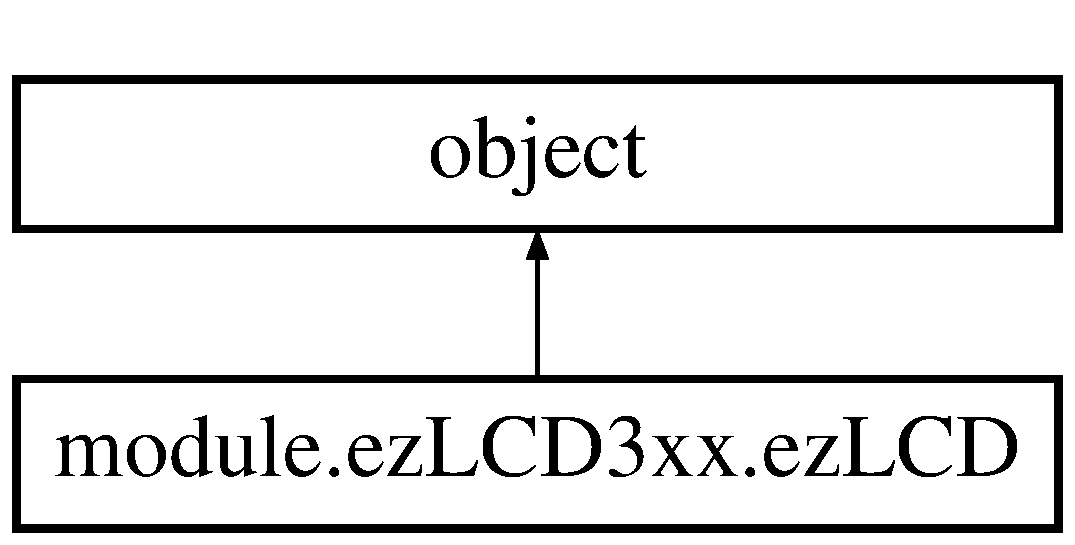
\includegraphics[height=2.000000cm]{d0/dec/classmodule_1_1ez_l_c_d3xx_1_1ez_l_c_d}
\end{center}
\end{figure}


The documentation for this class was generated from the following file\-:\begin{DoxyCompactItemize}
\item 
C\-:/\-Users/codeman/\-Documents/\-Git\-Hub/ez\-L\-C\-D3xx\-Python/module/ez\-L\-C\-D3xx.\-py\end{DoxyCompactItemize}

\chapter{Example Documentation}
\hypertarget{_button_align_8py-example}{\section{Button\-Align.\-py}
}

\begin{DoxyCodeInclude}
1 \textcolor{comment}{# Button Align ezLCD Python demo}
2 \textcolor{comment}{#}
3 
4 \textcolor{keyword}{import} platform
5 \textcolor{keyword}{import} sys
6 sys.path.append(\textcolor{stringliteral}{'..\(\backslash\)module'}) 
7 \textcolor{keyword}{from} ezLCD3xx \textcolor{keyword}{import} *
8 
9 \textcolor{comment}{#check what OS we are on}
10 \textcolor{comment}{#Windows}
11 \textcolor{keywordflow}{if} platform.system() == \textcolor{stringliteral}{'Windows'}:
12     LCD = ezLCD(\textcolor{stringliteral}{'com58'}) 
13 \textcolor{comment}{#Mac}
14 \textcolor{keywordflow}{elif} platform.system() == \textcolor{stringliteral}{'Dawrwin'}:
15     LCD = ezLCD(\textcolor{stringliteral}{'/dev/tty.usbsomething'})
16 \textcolor{comment}{#Linux}
17 \textcolor{keywordflow}{elif} platform.system() == \textcolor{stringliteral}{'Linux'}:
18     LCD = ezLCD(\textcolor{stringliteral}{'/dev/ttyACM0'})
19 
20 \textcolor{comment}{# Bail out if comport error}
21 \textcolor{keywordflow}{if} LCD.openSerial()==\textcolor{keyword}{False}:
22     \textcolor{keywordflow}{print} \textcolor{stringliteral}{'Error Opening Port'}
23     \textcolor{keywordflow}{raise} SystemExit
24 
25 \textcolor{comment}{# Turn verbose off }
26 LCD.verbose(\textcolor{stringliteral}{'off'})
27 \textcolor{comment}{# Turn off button press info from ezLCD}
28 LCD.wquiet(ON)
29 \textcolor{comment}{# CLear screen}
30 LCD.cls()
31 \textcolor{comment}{# Set draw color to red}
32 LCD.color(RED)
33 \textcolor{comment}{# Set widget font 0}
34 LCD.fontw(0,\textcolor{stringliteral}{'1'})
35 \textcolor{comment}{# Set wodget font 1}
36 LCD.fontw(1,\textcolor{stringliteral}{'0'})
37 \textcolor{comment}{# Set theme #1 }
38 LCD.theme(1, 155, 152, 3, 0, 3, 24, 4, 5, 0, 1)
39 \textcolor{comment}{# Draw button widget with a ID of 1}
40 LCD.color(WHITE)
41 LCD.printString(\textcolor{stringliteral}{'Button Alignment'},90,4)
42 LCD.color(RED)
43 LCD.xy(0,0)
44 LCD.box(319,239)
45 LCD.button( 1,  30,  25, 250, 30, 1, 0, 10, 6, 1,\textcolor{stringliteral}{'0 = Centered'})
46 LCD.button( 2,  30,  60, 250, 30, 1, 1, 10, 6, 2,\textcolor{stringliteral}{'1 = Right'})
47 LCD.button( 3,  30,  95, 250, 30, 1, 2, 10, 6, 3,\textcolor{stringliteral}{'2 = Left'})
48 LCD.button( 4,  30, 130, 250, 50, 1, 3, 10, 6, 4,\textcolor{stringliteral}{'3 = Bottom'})
49 LCD.button( 5,  30, 185, 250, 50, 1, 4, 10, 6, 5,\textcolor{stringliteral}{'4 = Top'})
\end{DoxyCodeInclude}
 
\hypertarget{_button_options_8py-example}{\section{Button\-Options.\-py}
}

\begin{DoxyCodeInclude}
1 \textcolor{comment}{# Button Options ezLCD Python demo}
2 \textcolor{comment}{#}
3 
4 \textcolor{keyword}{import} platform
5 \textcolor{keyword}{import} sys
6 sys.path.append(\textcolor{stringliteral}{'..\(\backslash\)module'}) 
7 \textcolor{keyword}{from} ezLCD3xx \textcolor{keyword}{import} *
8 
9 \textcolor{comment}{#check what OS we are on}
10 \textcolor{comment}{#Windows}
11 \textcolor{keywordflow}{if} platform.system() == \textcolor{stringliteral}{'Windows'}:
12     LCD = ezLCD(\textcolor{stringliteral}{'com4'}) 
13 \textcolor{comment}{#Mac}
14 \textcolor{keywordflow}{elif} platform.system() == \textcolor{stringliteral}{'Dawrwin'}:
15     LCD = ezLCD(\textcolor{stringliteral}{'/dev/tty.usbsomething'})
16 \textcolor{comment}{#Linux}
17 \textcolor{keywordflow}{elif} platform.system() == \textcolor{stringliteral}{'Linux'}:
18     LCD = ezLCD(\textcolor{stringliteral}{'/dev/ttyACM0'})
19 
20 \textcolor{comment}{# Bail out if comport error}
21 \textcolor{keywordflow}{if} LCD.openSerial()==\textcolor{keyword}{False}:
22     \textcolor{keywordflow}{print} \textcolor{stringliteral}{'Error Opening Port'}
23     \textcolor{keywordflow}{raise} SystemExit
24 
25 \textcolor{comment}{# Turn verbose off }
26 LCD.verbose(\textcolor{stringliteral}{'off'})
27 \textcolor{comment}{# Turn off button press info from ezLCD}
28 LCD.wquiet(ON)
29 \textcolor{comment}{# CLear screen}
30 LCD.cls()
31 \textcolor{comment}{# Set draw color to red}
32 LCD.color(RED)
33 \textcolor{comment}{# Set widget font 0}
34 LCD.fontw(0,\textcolor{stringliteral}{'1'})
35 \textcolor{comment}{# Set wodget font 1}
36 LCD.fontw(1,\textcolor{stringliteral}{'0'})
37 \textcolor{comment}{# Set theme #1 }
38 LCD.theme(1, 155, 152, 3, 0, 3, 24, 4, 5, 0, 1)
39 \textcolor{comment}{# Draw button widget with a ID of 1}
40 LCD.color(WHITE)
41 LCD.printString(\textcolor{stringliteral}{'Button Options'},90,4)
42 LCD.color(RED)
43 LCD.xy(0,0)
44 LCD.box(319,239)
45 LCD.button( 1,  30, 25, 250, 30, 1, 0, 10, 6, 3,\textcolor{stringliteral}{'1 = Draw'})
46 LCD.button( 2,  30, 60, 250, 30, 1, 0, 10, 6, 4,\textcolor{stringliteral}{'2 = Disabled'})
47 LCD.button( 3,  30, 95, 250, 30, 1, 0, 10, 6, 5,\textcolor{stringliteral}{'3 = Pressed'})
48 LCD.button( 4,  30, 130, 250, 30, 1, 0, 10, 6, 6,\textcolor{stringliteral}{'4 = Not Pressed'})
49 LCD.button( 5,  30, 165, 250, 30, 1, 0, 10, 6, 7,\textcolor{stringliteral}{'5 = Pressed Disabled'})
50 LCD.button( 6,  30, 200, 250, 30, 1, 0, 10, 6, 7,\textcolor{stringliteral}{'6 = Not Pressed Disabled'})
51 
52 
\end{DoxyCodeInclude}
 
\hypertarget{_button_radius_8py-example}{\section{Button\-Radius.\-py}
}

\begin{DoxyCodeInclude}
1 \textcolor{comment}{# Button Radius ezLCD Python demo}
2 \textcolor{comment}{#}
3 
4 \textcolor{keyword}{import} platform
5 \textcolor{keyword}{import} sys
6 sys.path.append(\textcolor{stringliteral}{'..\(\backslash\)module'}) 
7 \textcolor{keyword}{from} ezLCD3xx \textcolor{keyword}{import} *
8 
9 \textcolor{comment}{#check what OS we are on}
10 \textcolor{comment}{#Windows}
11 \textcolor{keywordflow}{if} platform.system() == \textcolor{stringliteral}{'Windows'}:
12     LCD = ezLCD(\textcolor{stringliteral}{'com4'}) 
13 \textcolor{comment}{#Mac}
14 \textcolor{keywordflow}{elif} platform.system() == \textcolor{stringliteral}{'Dawrwin'}:
15     LCD = ezLCD(\textcolor{stringliteral}{'/dev/tty.usbsomething'})
16 \textcolor{comment}{#Linux}
17 \textcolor{keywordflow}{elif} platform.system() == \textcolor{stringliteral}{'Linux'}:
18     LCD = ezLCD(\textcolor{stringliteral}{'/dev/ttyACM0'})
19 
20 \textcolor{comment}{# Bail out if comport error}
21 \textcolor{keywordflow}{if} LCD.openSerial()==\textcolor{keyword}{False}:
22     \textcolor{keywordflow}{print} \textcolor{stringliteral}{'Error Opening Port'}
23     \textcolor{keywordflow}{raise} SystemExit
24 
25 \textcolor{comment}{# Turn verbose off }
26 LCD.verbose(\textcolor{stringliteral}{'off'})
27 \textcolor{comment}{# Turn off button press info from ezLCD}
28 LCD.wquiet(ON)
29 \textcolor{comment}{# CLear screen}
30 LCD.cls()
31 \textcolor{comment}{# Set draw color to red}
32 LCD.color(RED)
33 \textcolor{comment}{# Set widget font 0}
34 LCD.fontw(0,\textcolor{stringliteral}{'1'})
35 \textcolor{comment}{# Set wodget font 1}
36 LCD.fontw(1,\textcolor{stringliteral}{'0'})
37 \textcolor{comment}{# Set theme #1 }
38 LCD.theme(1, 155, 152, 3, 0, 3, 24, 4, 5, 0, 1)
39 \textcolor{comment}{# Draw button widget with a ID of 1}
40 LCD.color(WHITE)
41 LCD.printString(\textcolor{stringliteral}{'Button Radius'},100,4)
42 LCD.color(RED)
43 LCD.xy(0,0)
44 LCD.box(319,239)
45 LCD.button( 1,  30, 25, 250, 30, 1, 0, 0, 6, 3,\textcolor{stringliteral}{'Radius = 0'})
46 LCD.button( 2,  30, 60, 250, 30, 1, 0, 10, 6, 4,\textcolor{stringliteral}{'Radius = 10'})
47 LCD.button( 3,  30, 95, 250, 30, 1, 0, 15, 6, 5,\textcolor{stringliteral}{'Radius = 15'})
48 LCD.button( 4,  30, 130, 100, 100, 1, 0, 20, 6, 6,\textcolor{stringliteral}{'Radius = 20'})
49 LCD.button( 5,  180, 130, 100, 100, 1, 0, 50, 6, 7,\textcolor{stringliteral}{'Radius = 50'})
50 
\end{DoxyCodeInclude}
 
\hypertarget{_touch_zone_i_m_8py-example}{\section{Touch\-Zone\-I\-M.\-py}
}

\begin{DoxyCodeInclude}
1 \textcolor{comment}{# Button Align ezLCD Python demo}
2 \textcolor{comment}{#}
3 
4 \textcolor{keyword}{import} platform
5 \textcolor{keyword}{import} sys
6 sys.path.append(\textcolor{stringliteral}{'..\(\backslash\)module'}) 
7 \textcolor{keyword}{from} ezLCD3xx \textcolor{keyword}{import} *
8 
9 \textcolor{comment}{#check what OS we are on}
10 \textcolor{comment}{#Windows}
11 \textcolor{keywordflow}{if} platform.system() == \textcolor{stringliteral}{'Windows'}:
12     LCD = ezLCD(\textcolor{stringliteral}{'com58'}) 
13 \textcolor{comment}{#Mac}
14 \textcolor{keywordflow}{elif} platform.system() == \textcolor{stringliteral}{'Dawrwin'}:
15     LCD = ezLCD(\textcolor{stringliteral}{'/dev/tty.usbsomething'})
16 \textcolor{comment}{#Linux}
17 \textcolor{keywordflow}{elif} platform.system() == \textcolor{stringliteral}{'Linux'}:
18     LCD = ezLCD(\textcolor{stringliteral}{'/dev/ttyACM0'})
19 
20 \textcolor{comment}{# Bail out if comport error}
21 \textcolor{keywordflow}{if} LCD.openSerial()==\textcolor{keyword}{False}:
22     \textcolor{keywordflow}{print} \textcolor{stringliteral}{'Error Opening Port'}
23     \textcolor{keywordflow}{raise} SystemExit
24 
25 tzData = ( 1, 0, 33,  2, 46, 33, 3, 92, 33, 4, 138, 33, 5, 184, 33, 6, 230, 33, 7, 276, 33, 
26            8, 0, 79, 9, 46, 79, 10, 92, 79, 11, 138, 79, 12, 184, 79, 13, 230, 79, 14, 276, 79,  
27           15, 0, 125, 16, 46, 125, 17, 92, 125, 18, 138, 125, 19, 184, 125, 20, 230, 125, 21, 276, 125) 
28 
29 \textcolor{comment}{# Turn verbose off }
30 LCD.verbose(\textcolor{stringliteral}{'off'})
31 \textcolor{comment}{# Turn off button press info from ezLCD}
32 LCD.wquiet(ON)
33 \textcolor{comment}{# CLear screen}
34 LCD.cls()
35 \textcolor{comment}{# Set draw color to red}
36 LCD.color(RED)
37 \textcolor{comment}{# Set widget font 0}
38 LCD.fontw(0,\textcolor{stringliteral}{'1'})
39 \textcolor{comment}{# Set wodget font 1}
40 LCD.fontw(1,\textcolor{stringliteral}{'0'})
41 \textcolor{comment}{# Set theme #1 }
42 LCD.theme(1, 155, 152, 3, 0, 3, 24, 4, 5, 0, 1)
43 \textcolor{comment}{# Draw button widget with a ID of 1}
44 LCD.picture(\textcolor{stringliteral}{'im.gif'}) \textcolor{comment}{# this will get a timeout error because it takes a bit to draw}
45 LCD.color(RED)
46 LCD.xy(0,0)
47 LCD.box(320,240)
48 LCD.printString(\textcolor{stringliteral}{'TouchZone Demo'}, 80, 10)
49 tzX = 0
50 tzY = 33
51 \textcolor{keywordflow}{for} count \textcolor{keywordflow}{in} range(0, 63, 3):
52     LCD.touchZone(tzData[count], tzData[count+1], tzData[count+2],43 ,43, ENABLE)
53 
54 \textcolor{keywordflow}{while} \textcolor{keyword}{True}:
55     (ID, Info, Data) = LCD.wstack(FIFO)
56     \textcolor{keywordflow}{if} ID > 0 \textcolor{keywordflow}{and} Info ==4:
57         ID -=1
58         LCD.color(BLACK)
59         LCD.xy(tzData[(ID*3)+1],tzData[(ID*3)+2] )
60         LCD.box(43,45)
61         string =\textcolor{stringliteral}{'TouchZone '} + str(ID+1) +\textcolor{stringliteral}{' Pressed'}
62         LCD.printString(string, 60, 200)
63     \textcolor{keywordflow}{if} ID > 0 \textcolor{keywordflow}{and} Info ==1 \textcolor{keywordflow}{or} Info ==2:
64         ID -=1
65         LCD.color(WHITE)        
66         LCD.xy(tzData[(ID*3)+1],tzData[(ID*3)+2] )
67         LCD.box(43,45)
68         LCD.printString(string, 60, 200)
69         
70 
\end{DoxyCodeInclude}
 
% Latex footer for doxygen 1.8.4
%--- End generated contents ---

% Index
\newpage
\phantomsection
\addcontentsline{toc}{part}{Index}
\printindex

\end{document}
